\subsection{Muon Fake Rate}
This section presents in more detail the studies on the muon fake rate.

\subsubsection{Fakeable Object}
The muon fakeable object definition is simply the muon selection requirements (Sec.~\ref{sec:sel_muons}) 
but with looser $d_0$ and isolation thresholds. We study the two definitions given 
in Section \ref{sec:fakerateDenominatorObjectDef}:
\begin{itemize}
  \item M1
  \begin{itemize}
    \item $|d_{0}| < 0.2$~cm
    \item $\frac{\rm{Iso}_{Total}}{\pt}~<~1.0$
  \end{itemize}
  \item M2 
  \begin{itemize}
    \item $|d_{0}| < 0.2$~cm
    \item $\frac{\rm{Iso}_{Total}}{\pt}~<~0.4$
  \end{itemize}
\end{itemize}
Note that M1 is the definition studied in~\cite{fakeLeptonNote2}. The motivation for the tighter selection 
of M2 is the reduction of systematic uncertainties by reducing the extrapolation in isolation.


\subsubsection{Calibration Sample Selection}
The muon fake rate has been measured in $192\ipb$ of data in Run2011A. The selected events are triggered
by any one of HLT\_Mu8 or HLT\_Mu15 single muon trigger paths. Addition requirements are also needed to
reduce contamination of the calibration sample with muons from $W$ and $Z$ decays and to tune the
jet composition:
\begin{itemize}
  \item $Z$ veto: reject the event if there are two oppositely charged muons satisfying the loose muon 
        selection and with $p_T>20\:\GeVc$,
  \item $W$ veto: reject the event if PF-MET $> 20\:\GeV$ or if the transverse mass of the loose muon 
        and PF-MET is above $20\:\GeVcc$,
  \item require the presence of a PF-jet with $p_T > 15\:\GeVc$ and separated by $\Delta R > 1$ 
        from the loose muon.
\end{itemize}
The jet threshold of $p_T > 15\:\GeVc$, corrected for the contribution of pileup, was found to best model 
the jet spectrum of the $W+$jets process described in more detail in Section 
\ref{sec:FakeMuonBkgJetSpectrumSystematics} below. The jets used in this study have the L1FastJet, 
L2Relative, and L3Absolute jet energy corrections applied. 


\subsubsection{Fake Rates}
The fake rate parametrized in $\eta$-$p_T$ is listed in Tabs.~\ref{tab:mu_fr_iso1_jet15} and~\ref{tab:mu_fr_iso04_jet15}. 
Figs.~\ref{fig:mu_fr_iso1_jet15} and~\ref{fig:mu_fr_iso04_jet15} show how the fake rates trends when projected onto $p_T$ or $\eta$.



\begin{table}[!htbp]
\begin{center}
\begin{tabular}{|c|c|c|c|c|}

\hline
                       &        $ 0<\eta<=1.0$            &        $1.0<\eta<=1.479$         &        $1.479<\eta<=2.0$         &        $2.0<\eta<=2.4$            \\
\hline
    $10 < p_{T} <= 15$ &        $0.098^{+0.002}_{-0.002}$ &        $0.114^{+0.003}_{-0.003}$ &        $0.133^{+0.003}_{-0.003}$ &        $0.161^{+0.005}_{-0.005}$  \\ 
 \hline
    $15 < p_{T} <= 20$ &        $0.064^{+0.001}_{-0.001}$ &        $0.085^{+0.001}_{-0.001}$ &        $0.103^{+0.001}_{-0.001}$ &        $0.132^{+0.002}_{-0.002}$  \\ 
 \hline
    $20 < p_{T} <= 25$ &        $0.114^{+0.001}_{-0.001}$ &        $0.153^{+0.002}_{-0.002}$ &        $0.151^{+0.003}_{-0.003}$ &        $0.205^{+0.006}_{-0.006}$  \\ 
 \hline
    $25 < p_{T} <= 30$ &        $0.098^{+0.002}_{-0.002}$ &        $0.141^{+0.004}_{-0.004}$ &        $0.143^{+0.005}_{-0.005}$ &        $0.204^{+0.011}_{-0.011}$  \\ 
 \hline
    $30 < p_{T} <= 35$ &        $0.095^{+0.004}_{-0.004}$ &        $0.126^{+0.007}_{-0.007}$ &        $0.138^{+0.008}_{-0.008}$ &        $0.187^{+0.021}_{-0.019}$  \\ 
 \hline
\end{tabular}
\caption{Muon fake rate in $\eta$-$p_T$ for the M1 fakeable object definition. Uncertainties are statistical only.
The {\bf Mu8} triggers are used, with a $p_{T}$ threshold on the leading jet in the event of $15$ GeV. }
\label{tab:mu_fr_M2_jet15}
\end{center}
\end{table}






\begin{table}[!htbp]
\begin{center}
\begin{tabular}{|c|c|c|c|c|}

\hline
                       &        $ 0<\eta<=1.0$            &        $1.0<\eta<=1.479$         &        $1.479<\eta<=2.0$         &        $2.0<\eta<=2.4$            \\
\hline
    $10 < p_{T} <= 15$ &        $0.182^{+0.003}_{-0.003}$ &        $0.199^{+0.005}_{-0.005}$ &        $0.217^{+0.005}_{-0.005}$ &        $0.244^{+0.007}_{-0.007}$  \\ 
 \hline
    $15 < p_{T} <= 20$ &        $0.130^{+0.001}_{-0.001}$ &        $0.153^{+0.002}_{-0.002}$ &        $0.170^{+0.002}_{-0.002}$ &        $0.200^{+0.003}_{-0.003}$  \\ 
 \hline
    $20 < p_{T} <= 25$ &        $0.250^{+0.003}_{-0.003}$ &        $0.284^{+0.004}_{-0.004}$ &        $0.255^{+0.004}_{-0.004}$ &        $0.311^{+0.008}_{-0.008}$  \\ 
 \hline
    $25 < p_{T} <= 30$ &        $0.226^{+0.005}_{-0.005}$ &        $0.277^{+0.008}_{-0.008}$ &        $0.245^{+0.008}_{-0.008}$ &        $0.311^{+0.016}_{-0.016}$  \\ 
 \hline
    $30 < p_{T} <= 35$ &        $0.235^{+0.009}_{-0.008}$ &        $0.258^{+0.014}_{-0.013}$ &        $0.240^{+0.014}_{-0.013}$ &        $0.287^{+0.030}_{-0.028}$  \\ 
 \hline
\end{tabular}
\caption{Muon fake rate in $\eta$-$p_T$ for the M2 fakeable object definition. Uncertainties are statistical only.
The {\bf Mu8} triggers are used, with a $p_{T}$ threshold on the leading jet in the event of $15$ GeV. }
\label{tab:mu_fr_M2_jet15}
\end{center}
\end{table}





\begin{figure}[!htbp]
\begin{center}
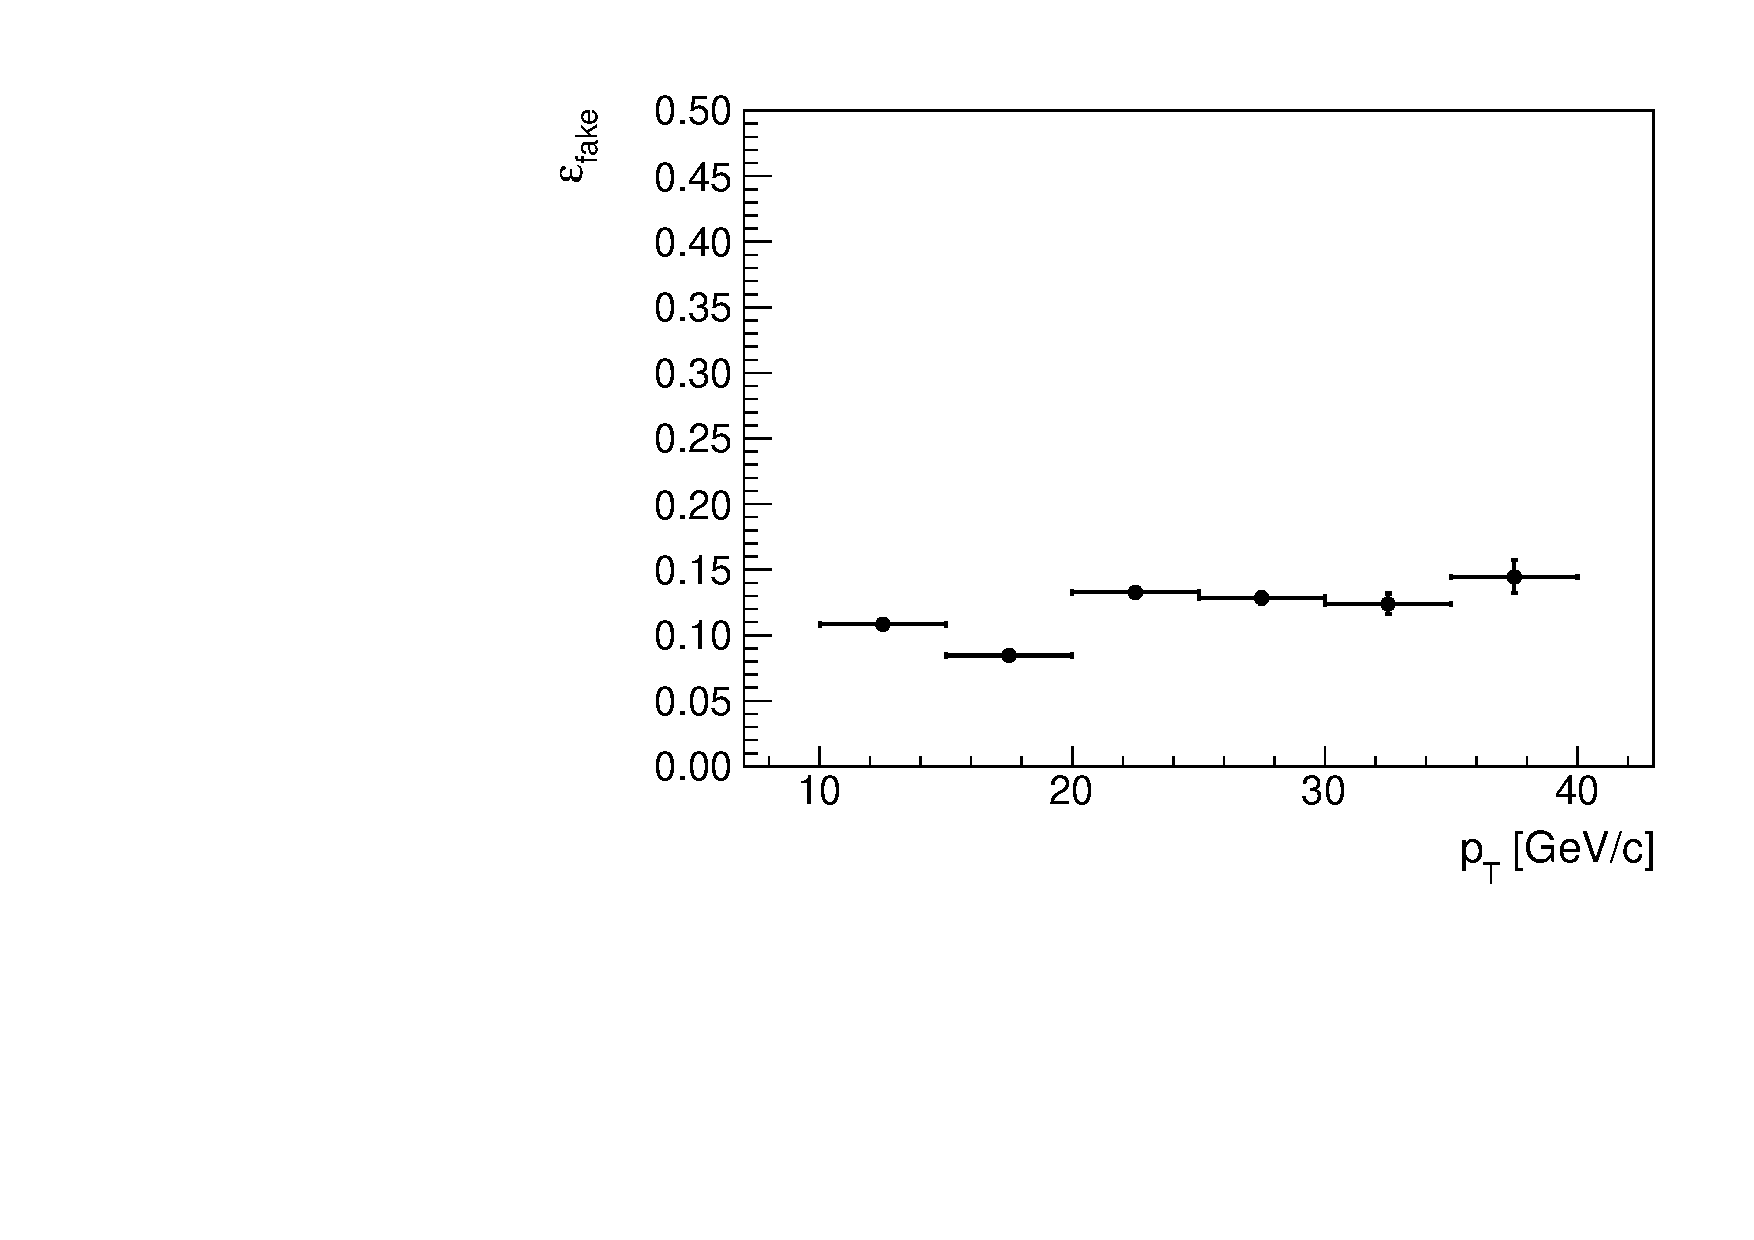
\includegraphics[width=0.45\textwidth]{figures/muon_frpt_m1.pdf}
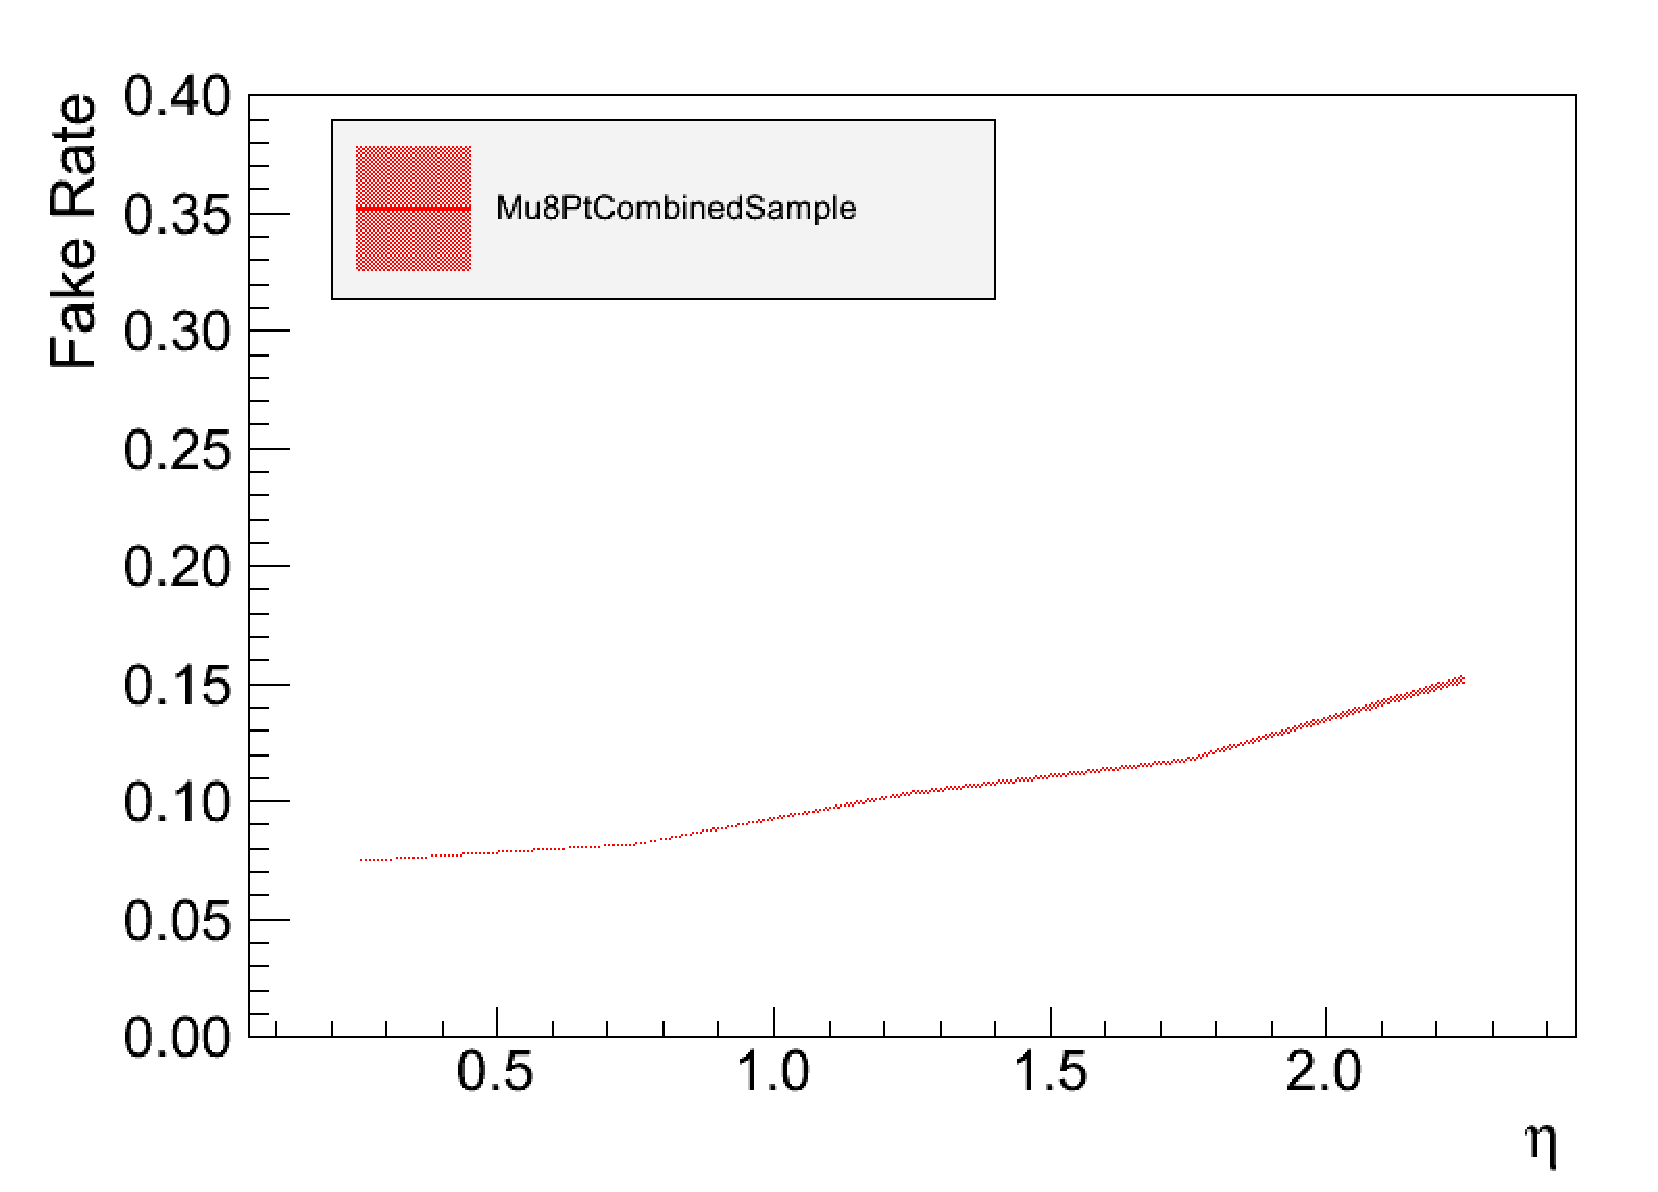
\includegraphics[width=0.45\textwidth]{figures/muon_freta_m1.pdf}
\caption{Fake rates for M1 definition projected onto $p_T$ and $\eta$.}
\label{fig:mu_fr_iso1_jet15}
\end{center}
\end{figure}

\begin{figure}[!htbp]
\begin{center}
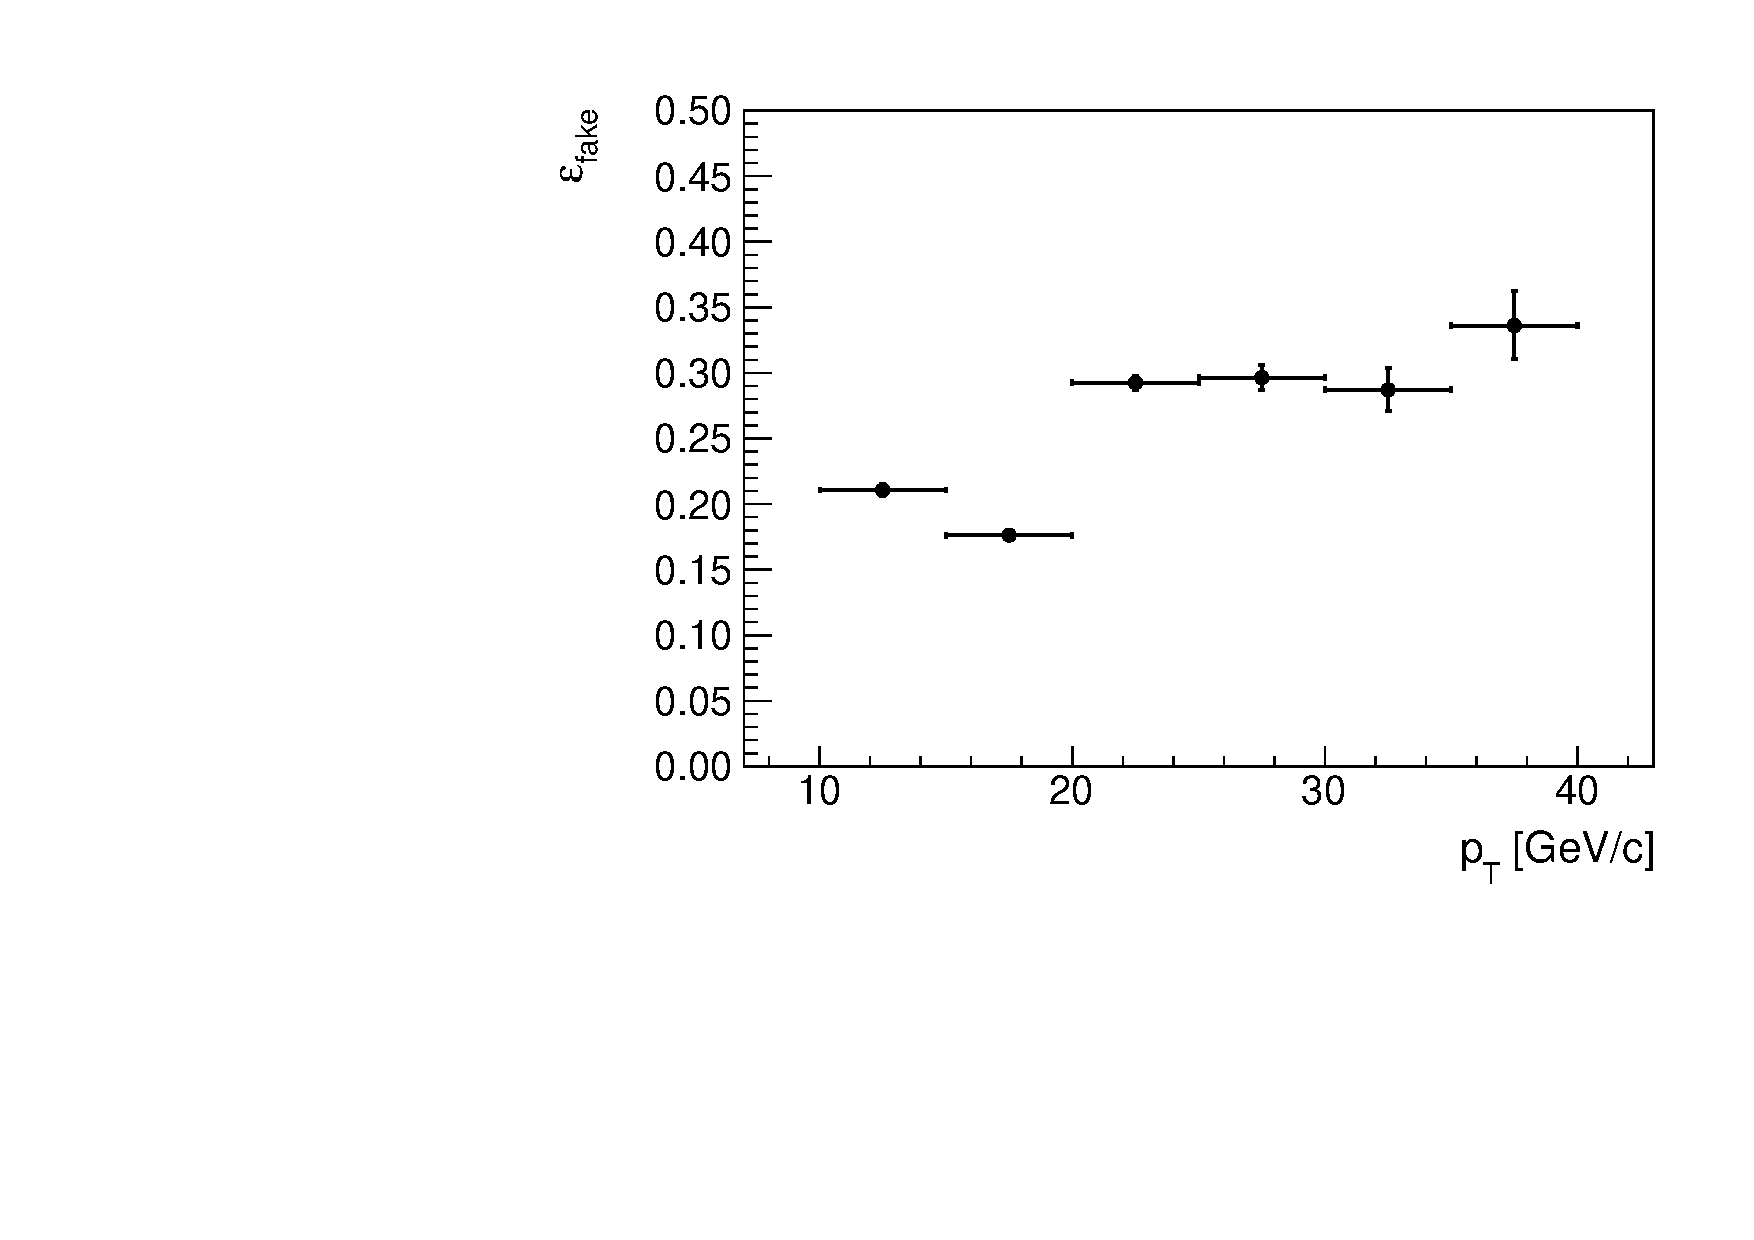
\includegraphics[width=0.45\textwidth]{figures/muon_frpt_m2.pdf}
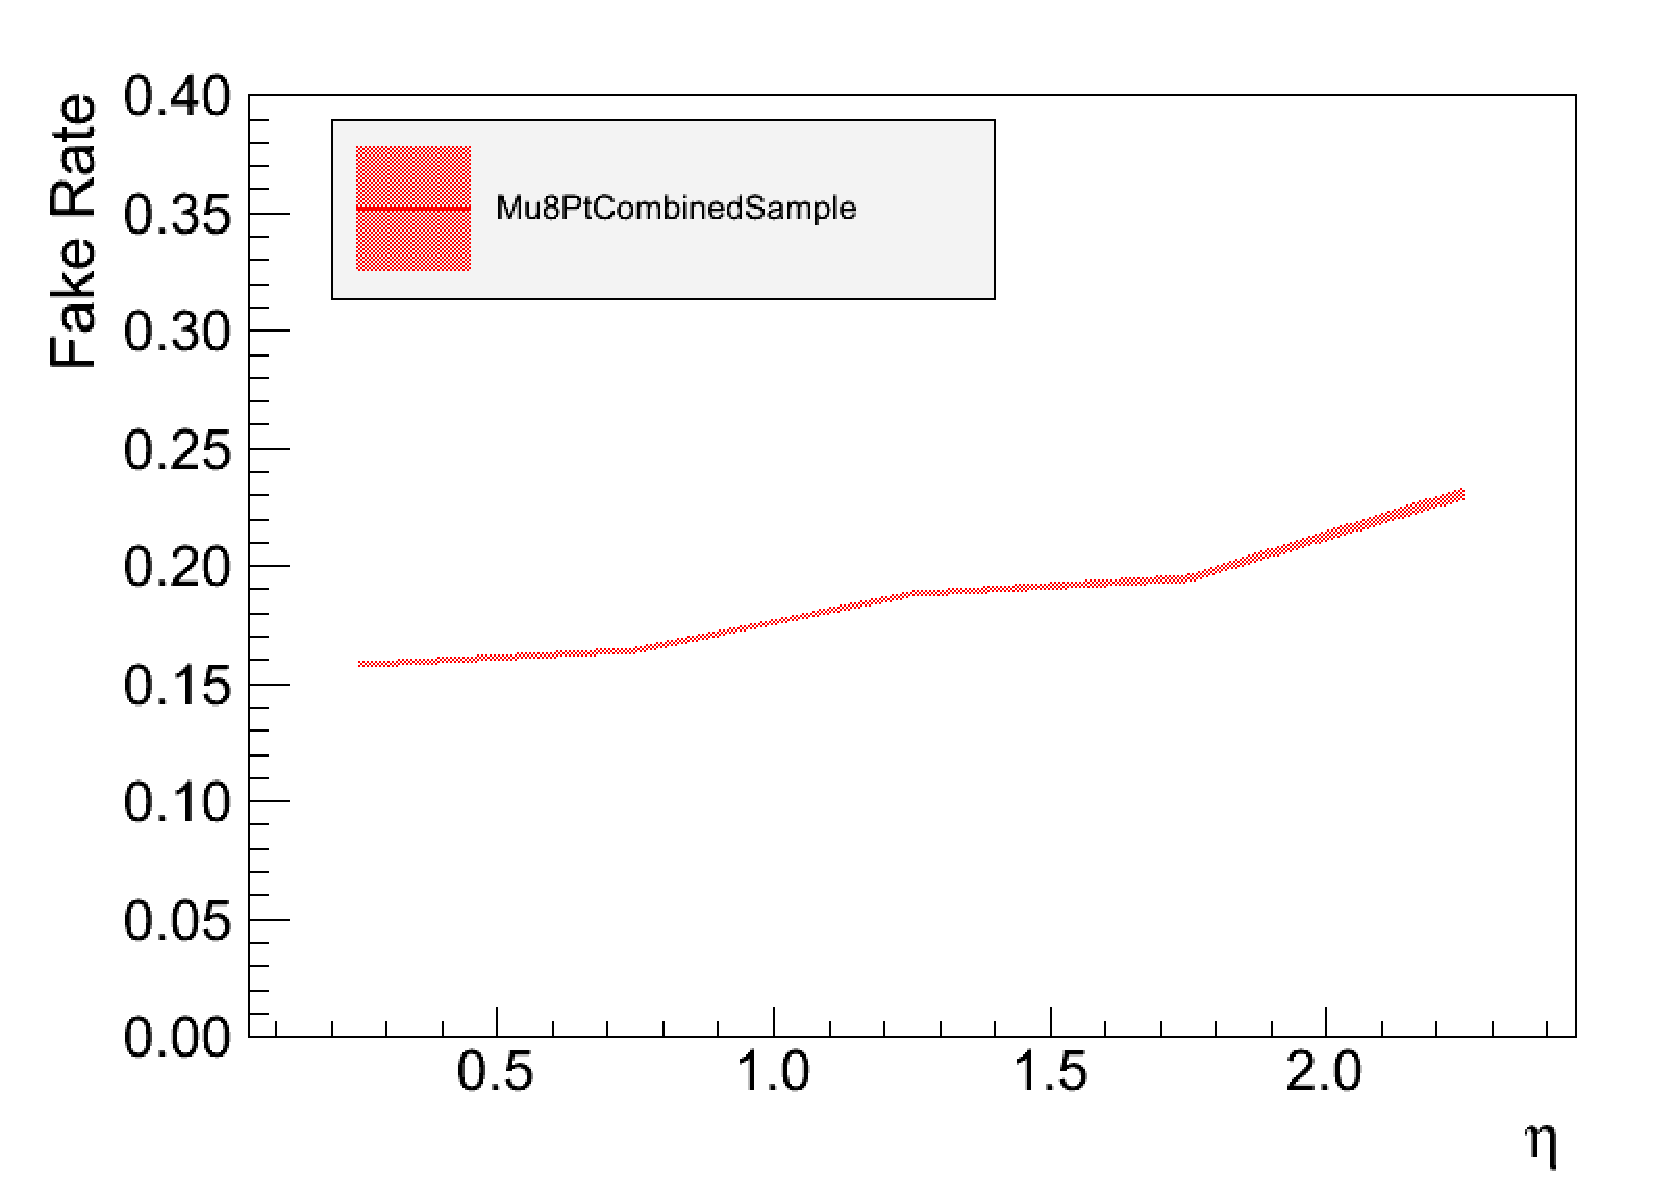
\includegraphics[width=0.45\textwidth]{figures/muon_freta_m2.pdf}
\caption{Fake rates for M2 definition projected onto $p_T$ and $\eta$.}
\label{fig:mu_fr_iso04_jet15}
\end{center}
\end{figure}


\subsubsection{Jet $p_{T}$ Spectrum Systematics}
\label{sec:FakeMuonBkgJetSpectrumSystematics}

The isolation efficiency for fake muons are affected by any difference of the spectrum of the
jet that a fakeable object lies inside between the fake rate measurement sample and the 
application sample. To study this systematic uncertainty, we compare the $p_{T}$ spectrum 
of the jet that a particular fakeable object lies inside for the W+Jet Monte Carlo sample and the
data sample in which we measure the fake rates. This spectrum is representative of the $p_{T}$
spectrum of a particular parton which produces the fake muon after fragmentation and 
hadronization. Figures \ref{fig:mu_M1_fr_jetspectrum0To30} and \ref{fig:mu_M2_fr_jetspectrum0To30} show 
this comparison between the W+Jet spectrum and the spectrum obtained from the fake rate measurement 
sample in data for three different thresholds on the leading jet in the event, for the M1 and M2
fakeable object definitions respectively. Ideally one wants to match the data spectrum to the
W+Jet spectrum to obtain an unbiased fake rate determination, however none of our data-based
samples matches completely. The sample obtained with a threshold on the leading jet of
$15$ GeV matches the W+Jet spectrum the best, and is taken for the central value of the 
fake rate measurement. The systematic uncertainty is estimated by using fake rates from the sample 
defined by thresholds of $0$ and $30$ GeV, since they are observed to cover the 
correct W+Jet spectrum. Figures \ref{fig:mu_M1_fr_jetspectrumNarrowerWindow} and 
\ref{fig:mu_M2_fr_jetspectrumNarrowerWindow} show analogous 
comparisons of the jet spectrum with narrower windows on the leading jet $p_{T}$ threshold 
for the M1 and M2 denominator definitions respectively, providing some guidance on the 
possibility for more aggressive systematic uncertainty estimates.

Table \ref{tab:mu_fr_JetSpectrumSystematics} summarizes the systematic
uncertainties due to the jet spectrum. The systematic uncertainties from the M1 extrapolation
is about $10\%$ larger than the systematic uncertainties from the M2 extrapolation. 
Using the M2 extrapolation, we estimate a systematic uncertainty of $31\%$, taking the largest 
difference between the $0$GeV threshold result and the $30$ GeV threshold result after the 
WW selection.

\begin{figure}[!htbp]
\begin{center}
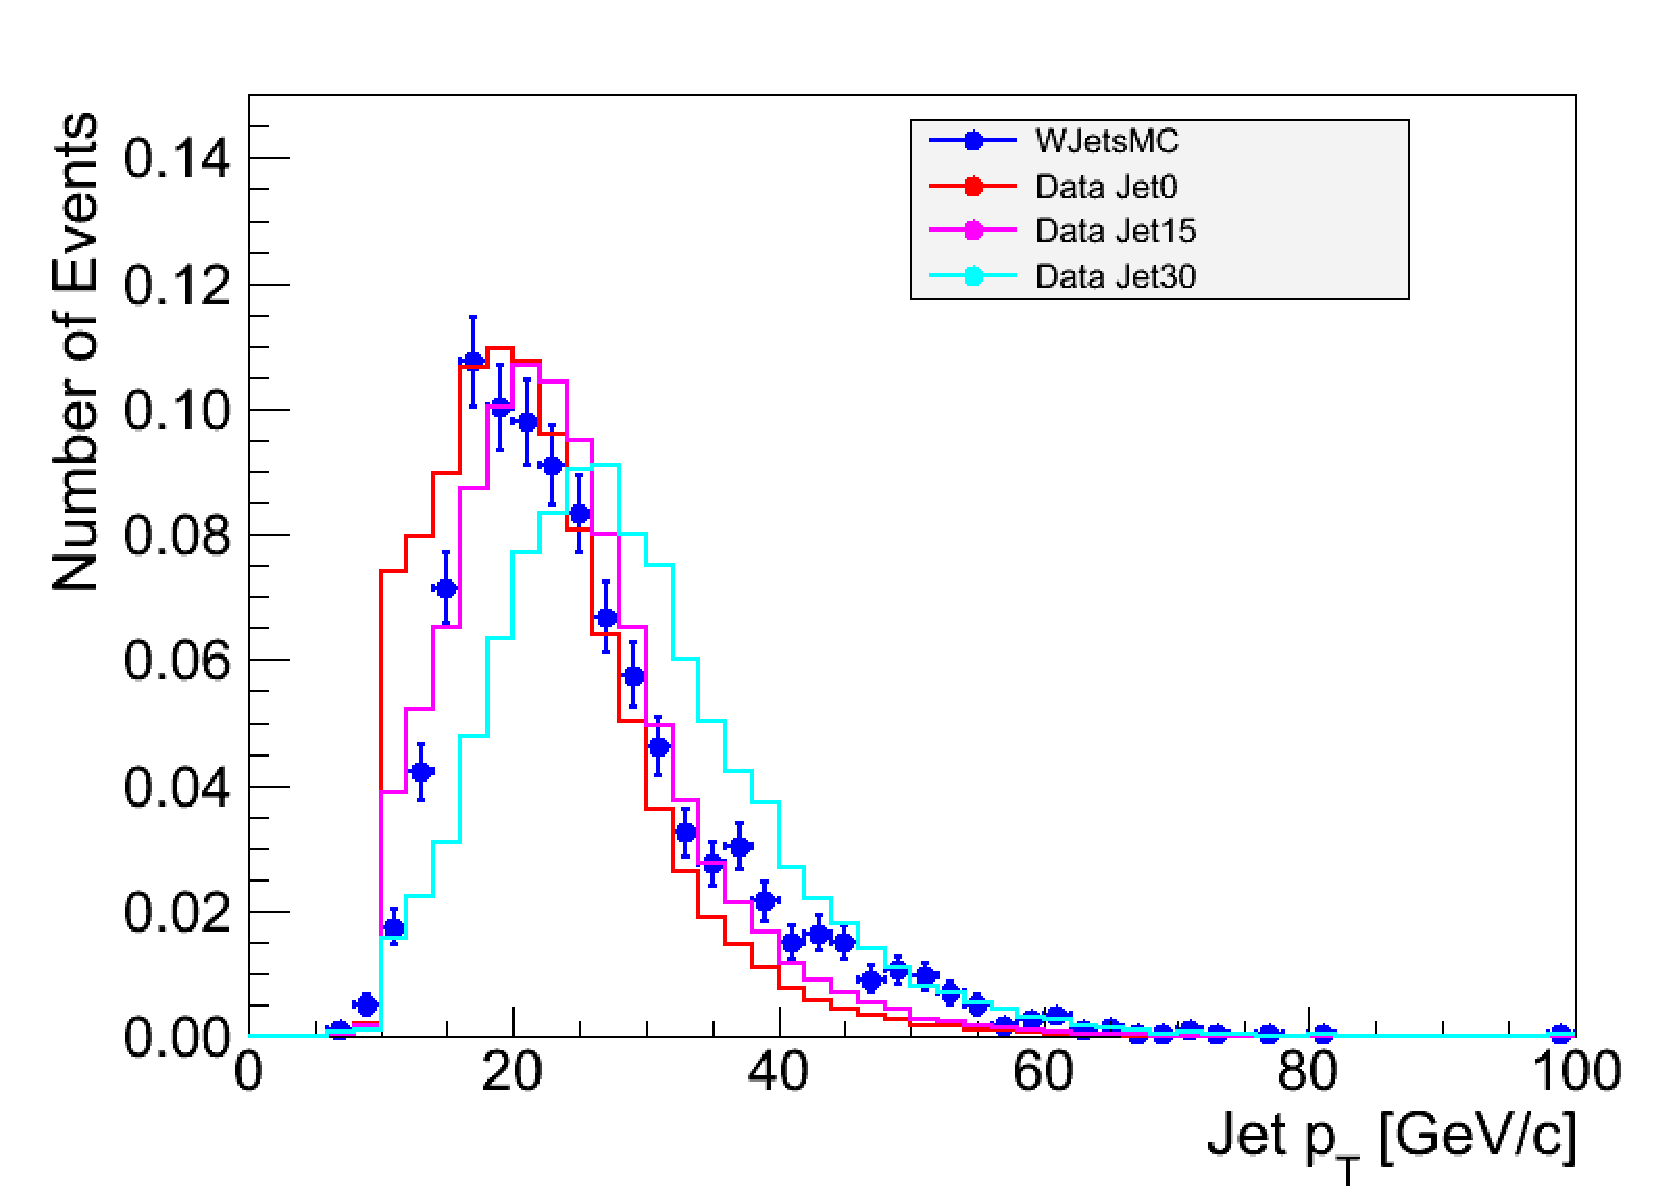
\includegraphics[width=0.75\textwidth]{figures/LeptonJetPt_MuonM1_0To30.pdf}
\caption{The $p_{T}$ spectrum of the jet that a M1 muon fakeable object lies inside for the 
W+Jet Monte Carlo sample and the data fake rate measurement sample, requiring a threshold on the $p_{T}$ of 
the leading jet in the event between $0$ and $30$ GeV.}
\label{fig:mu_M1_fr_jetspectrum0To30}
\end{center}
\end{figure}

\begin{figure}[!htbp]
\begin{center}
\subfigure[$p_{T}$ Threshold : $5-25$ GeV]{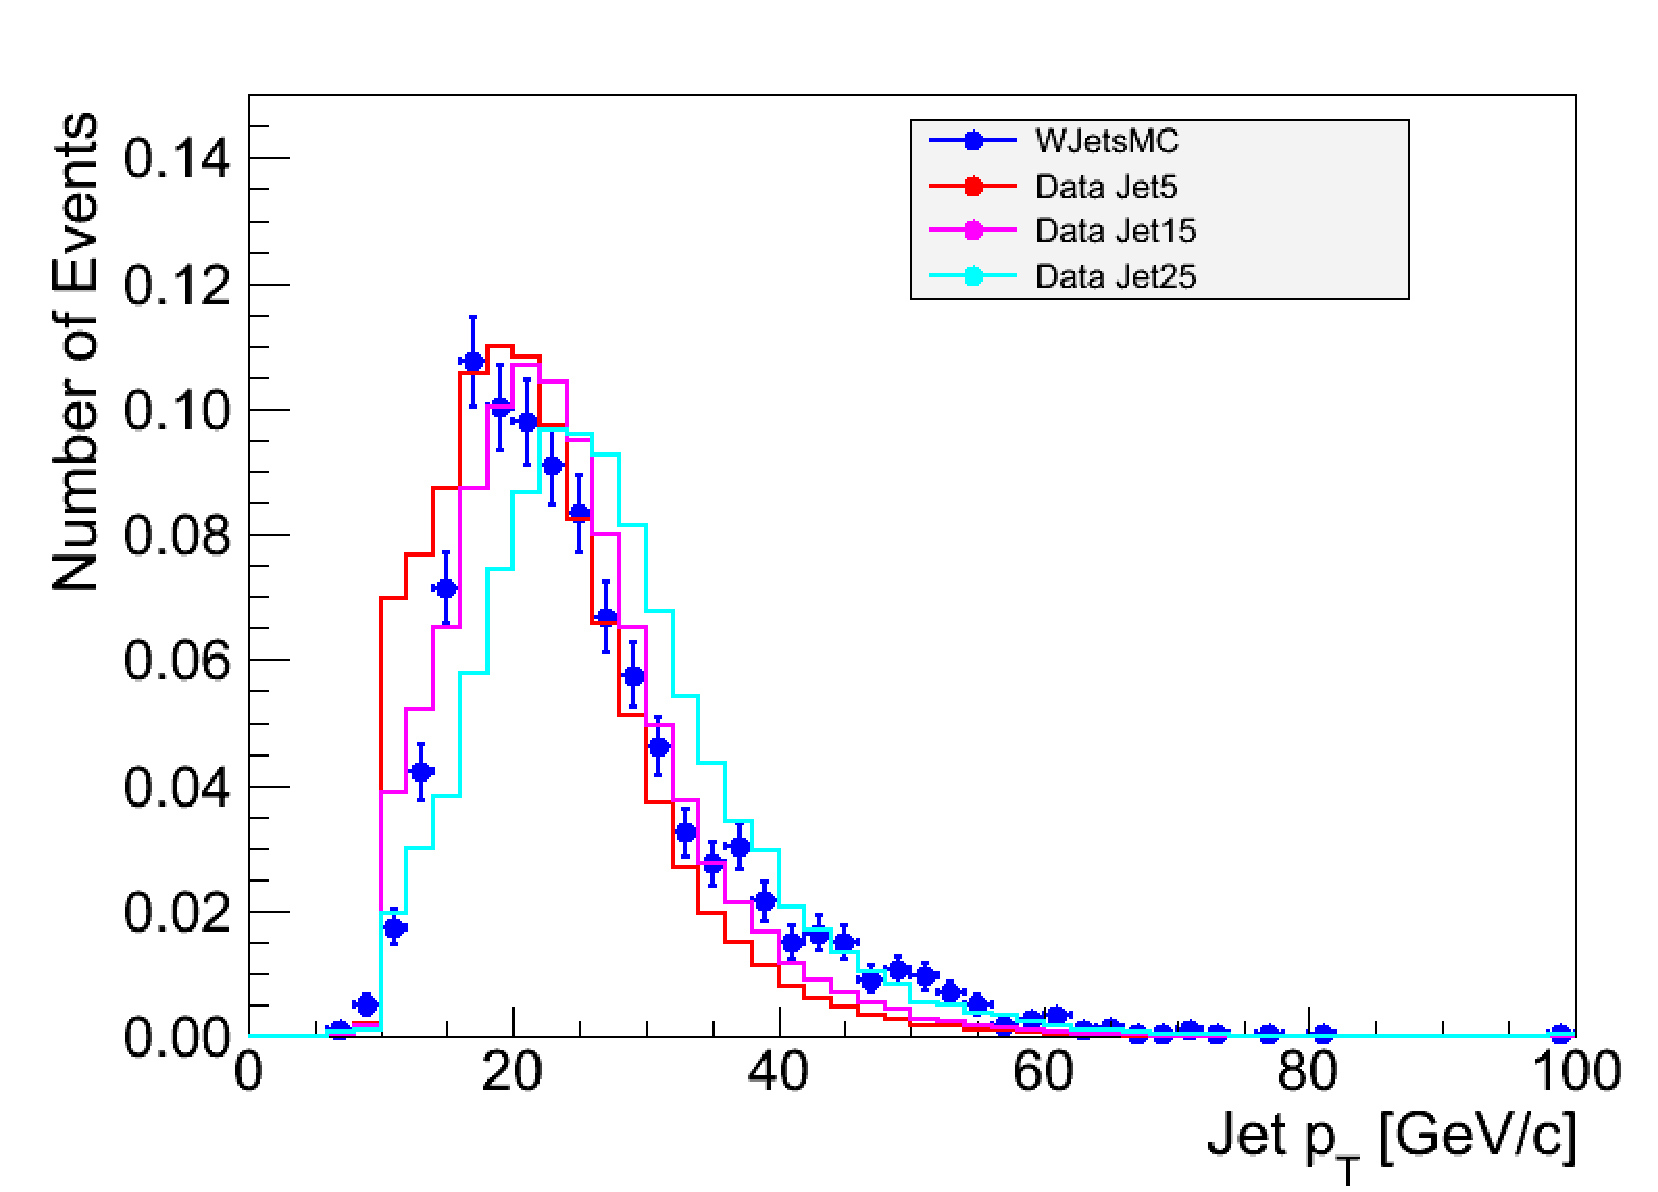
\includegraphics[width=0.45\textwidth]{figures/LeptonJetPt_MuonM1_5To25.pdf}}
\subfigure[$p_{T}$ Threshold : $10-20$ GeV]{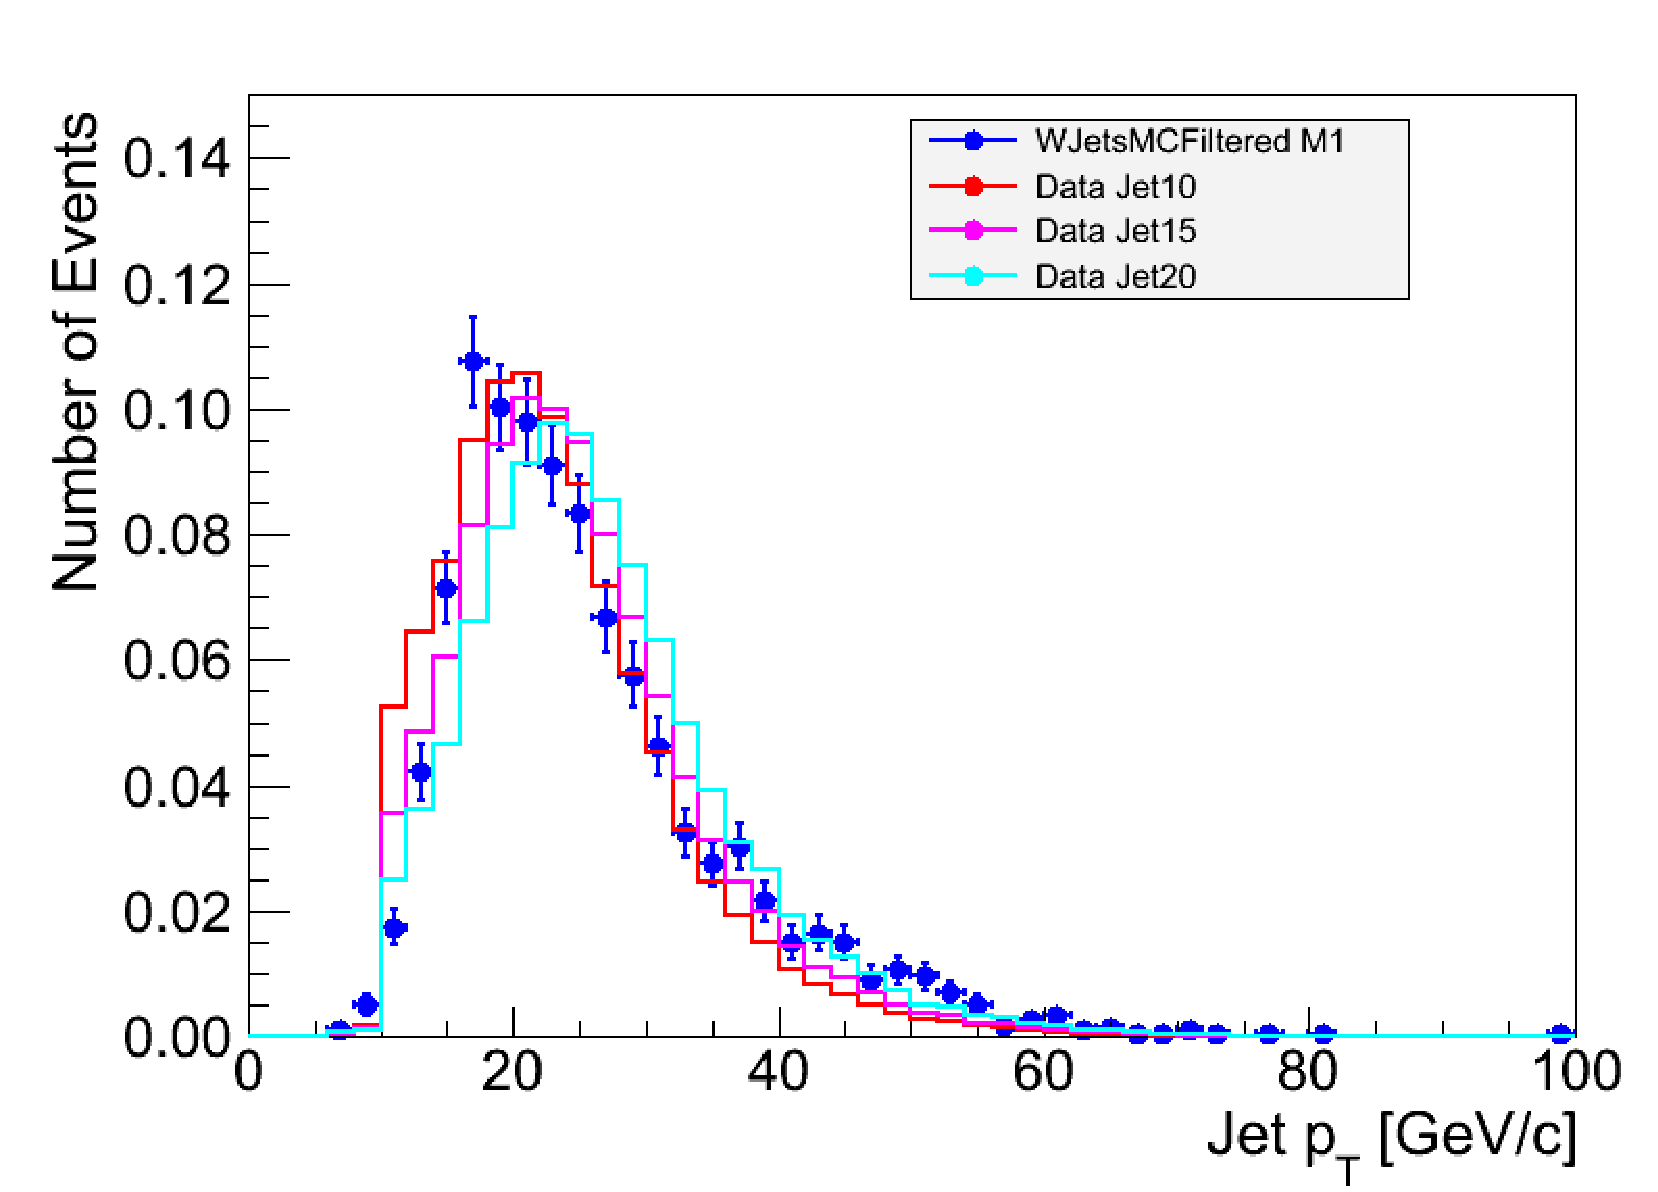
\includegraphics[width=0.45\textwidth]{figures/LeptonJetPt_MuonM1_10To20.pdf}}
\caption{The $p_{T}$ spectrum of the jet that a M1 muon fakeable object lies inside for the 
W+Jet Monte Carlo sample and the data fake rate measurement sample, for a narrower window of thresholds
on the $p_{T}$ of the leading jet in the event.}
\label{fig:mu_M1_fr_jetspectrumNarrowerWindow}
\end{center}
\end{figure}

\begin{figure}[!htbp]
\begin{center}
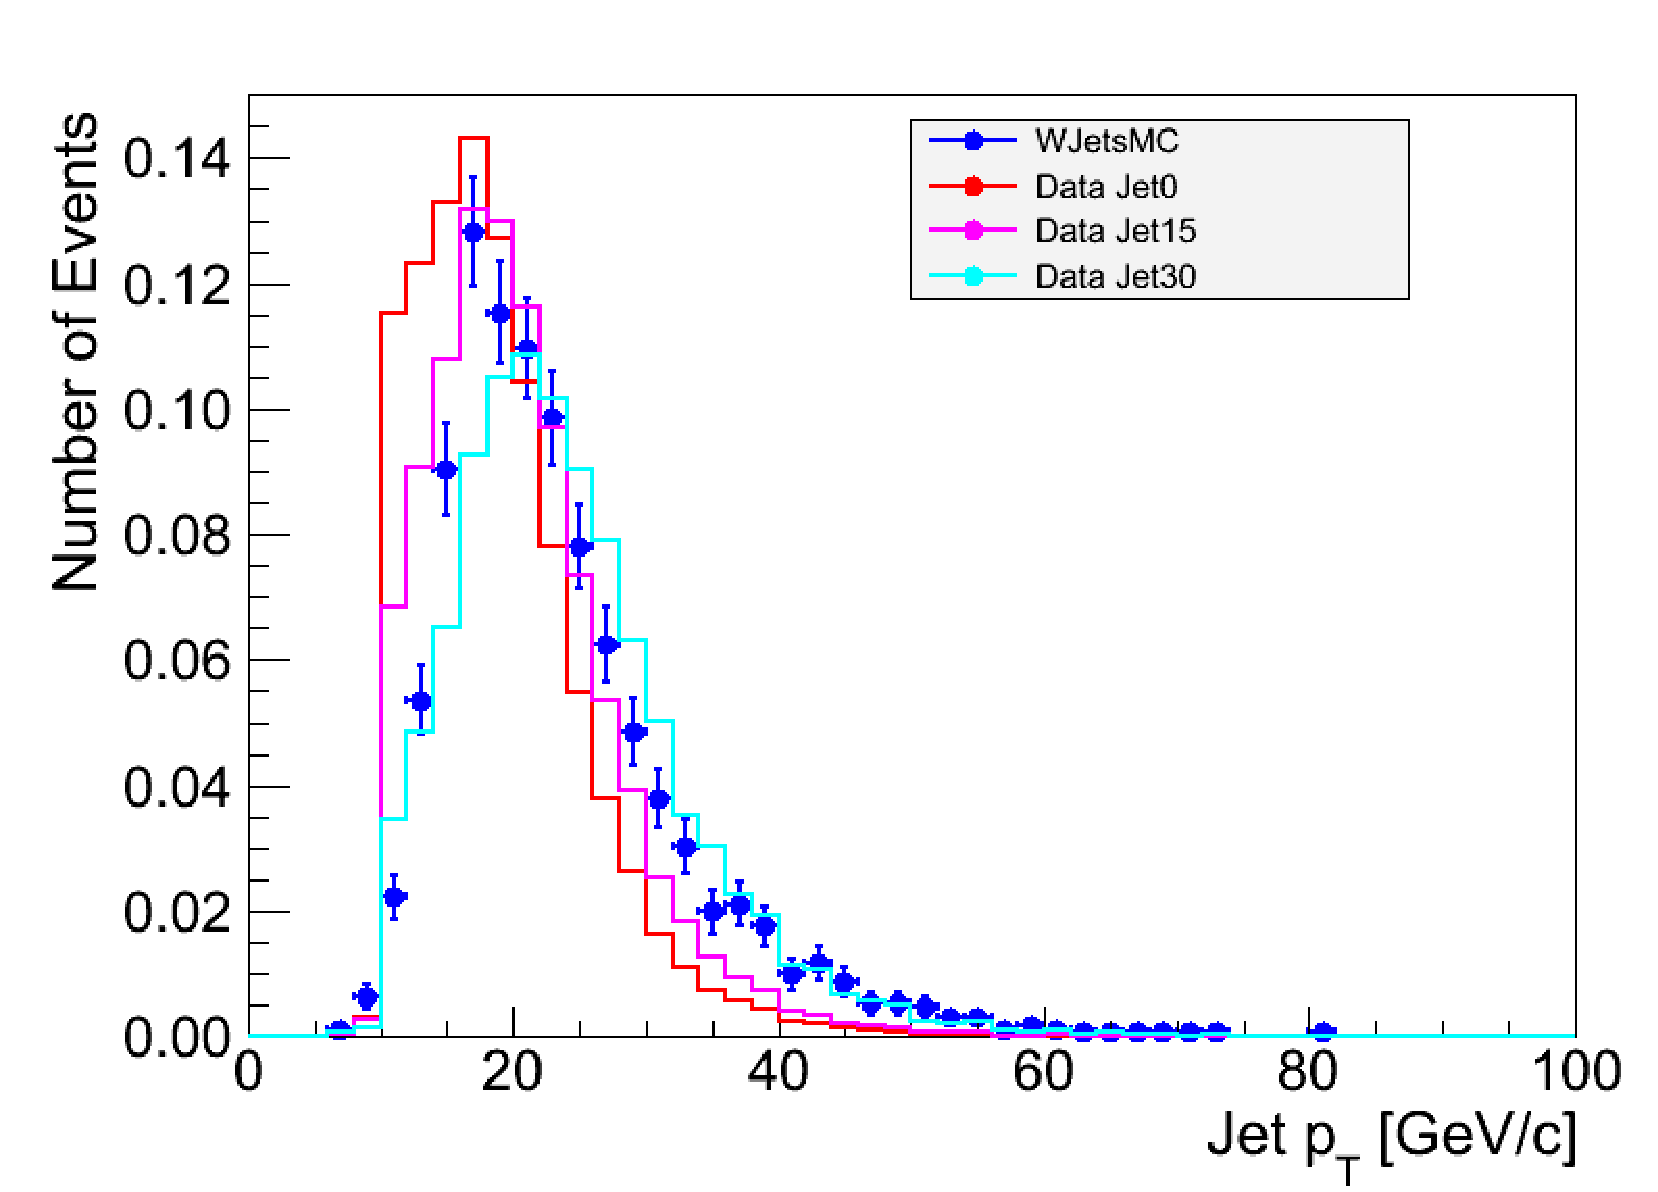
\includegraphics[width=0.75\textwidth]{figures/LeptonJetPt_MuonM2_0To30.pdf}
\caption{The $p_{T}$ spectrum of the jet that a M2 muon fakeable object lies inside for the 
W+Jet Monte Carlo sample and the data fake rate measurement sample, requiring a threshold on the $p_{T}$ of 
the leading jet in the event between $0$ and $30$ GeV.}
\label{fig:mu_M2_fr_jetspectrum0To30}
\end{center}
\end{figure}

\begin{figure}[!htbp]
\begin{center}
\subfigure[$p_{T}$ Threshold : $5-25$ GeV]{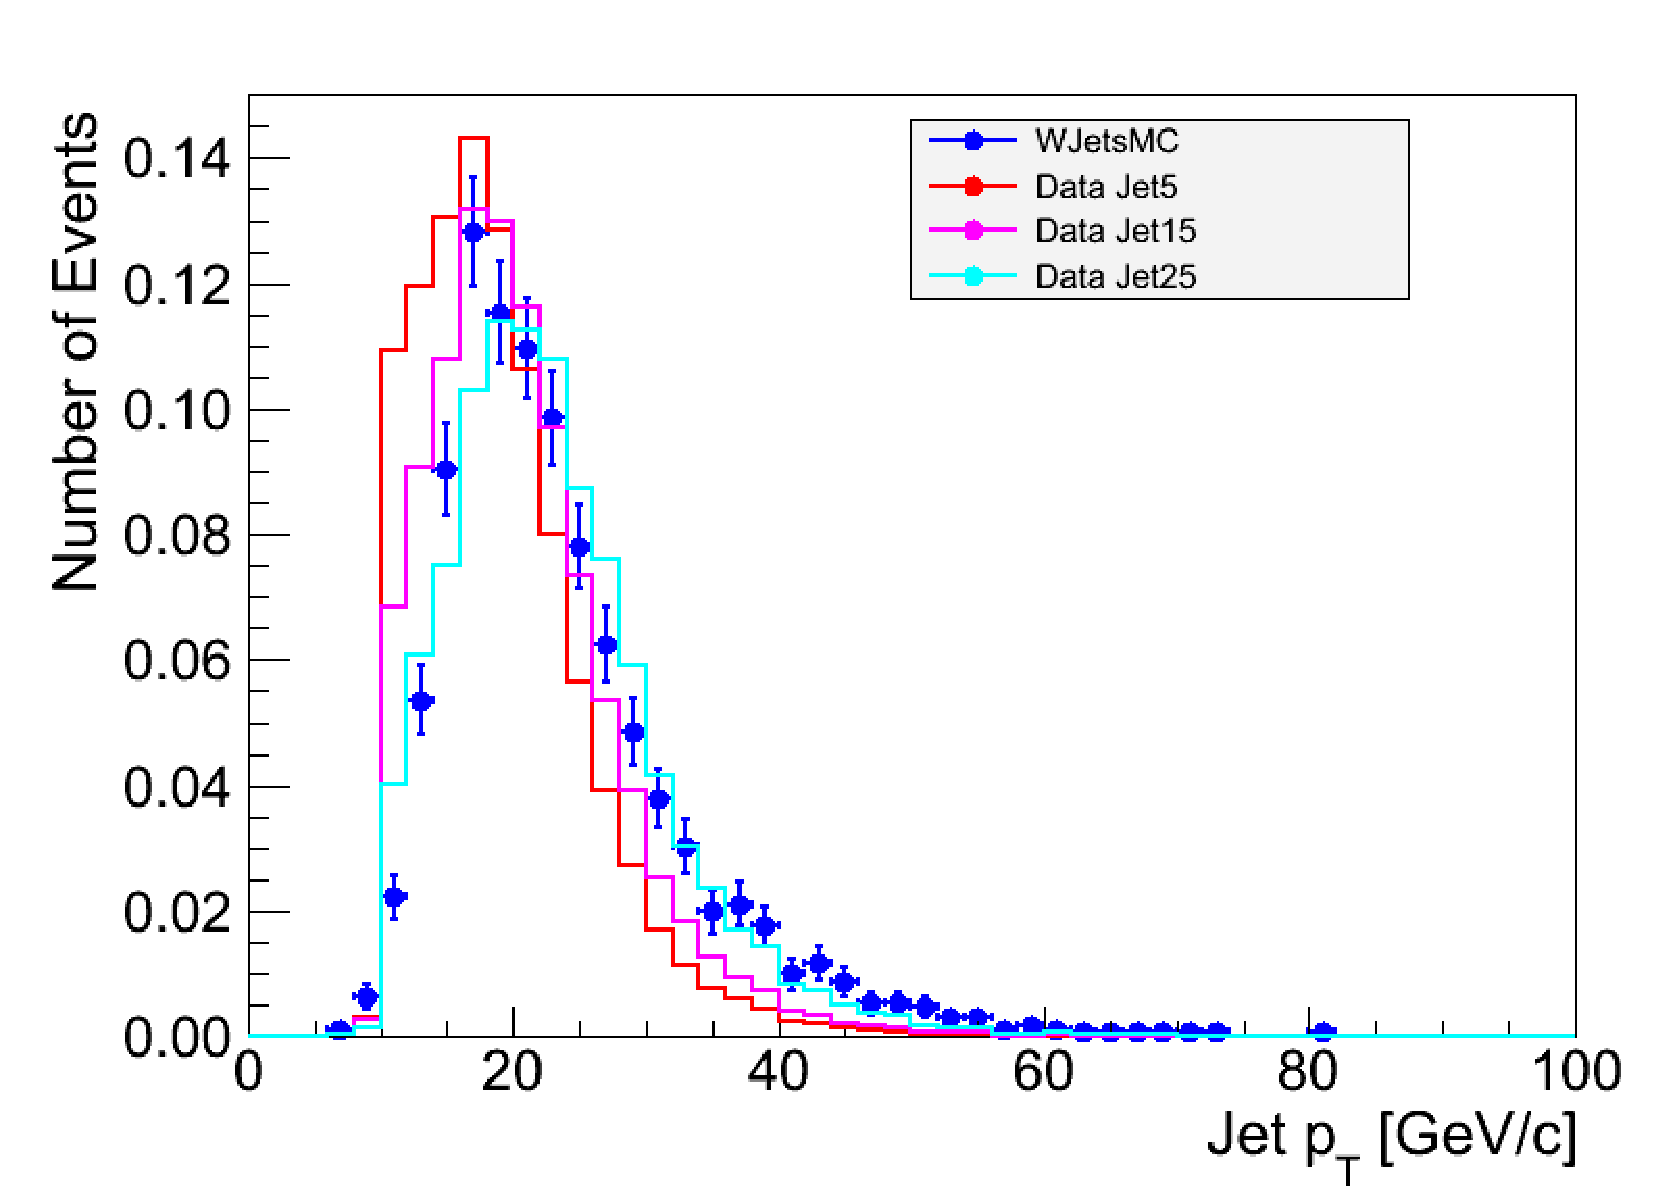
\includegraphics[width=0.45\textwidth]{figures/LeptonJetPt_MuonM2_5To25.pdf}}
\subfigure[$p_{T}$ Threshold : $10-20$ GeV]{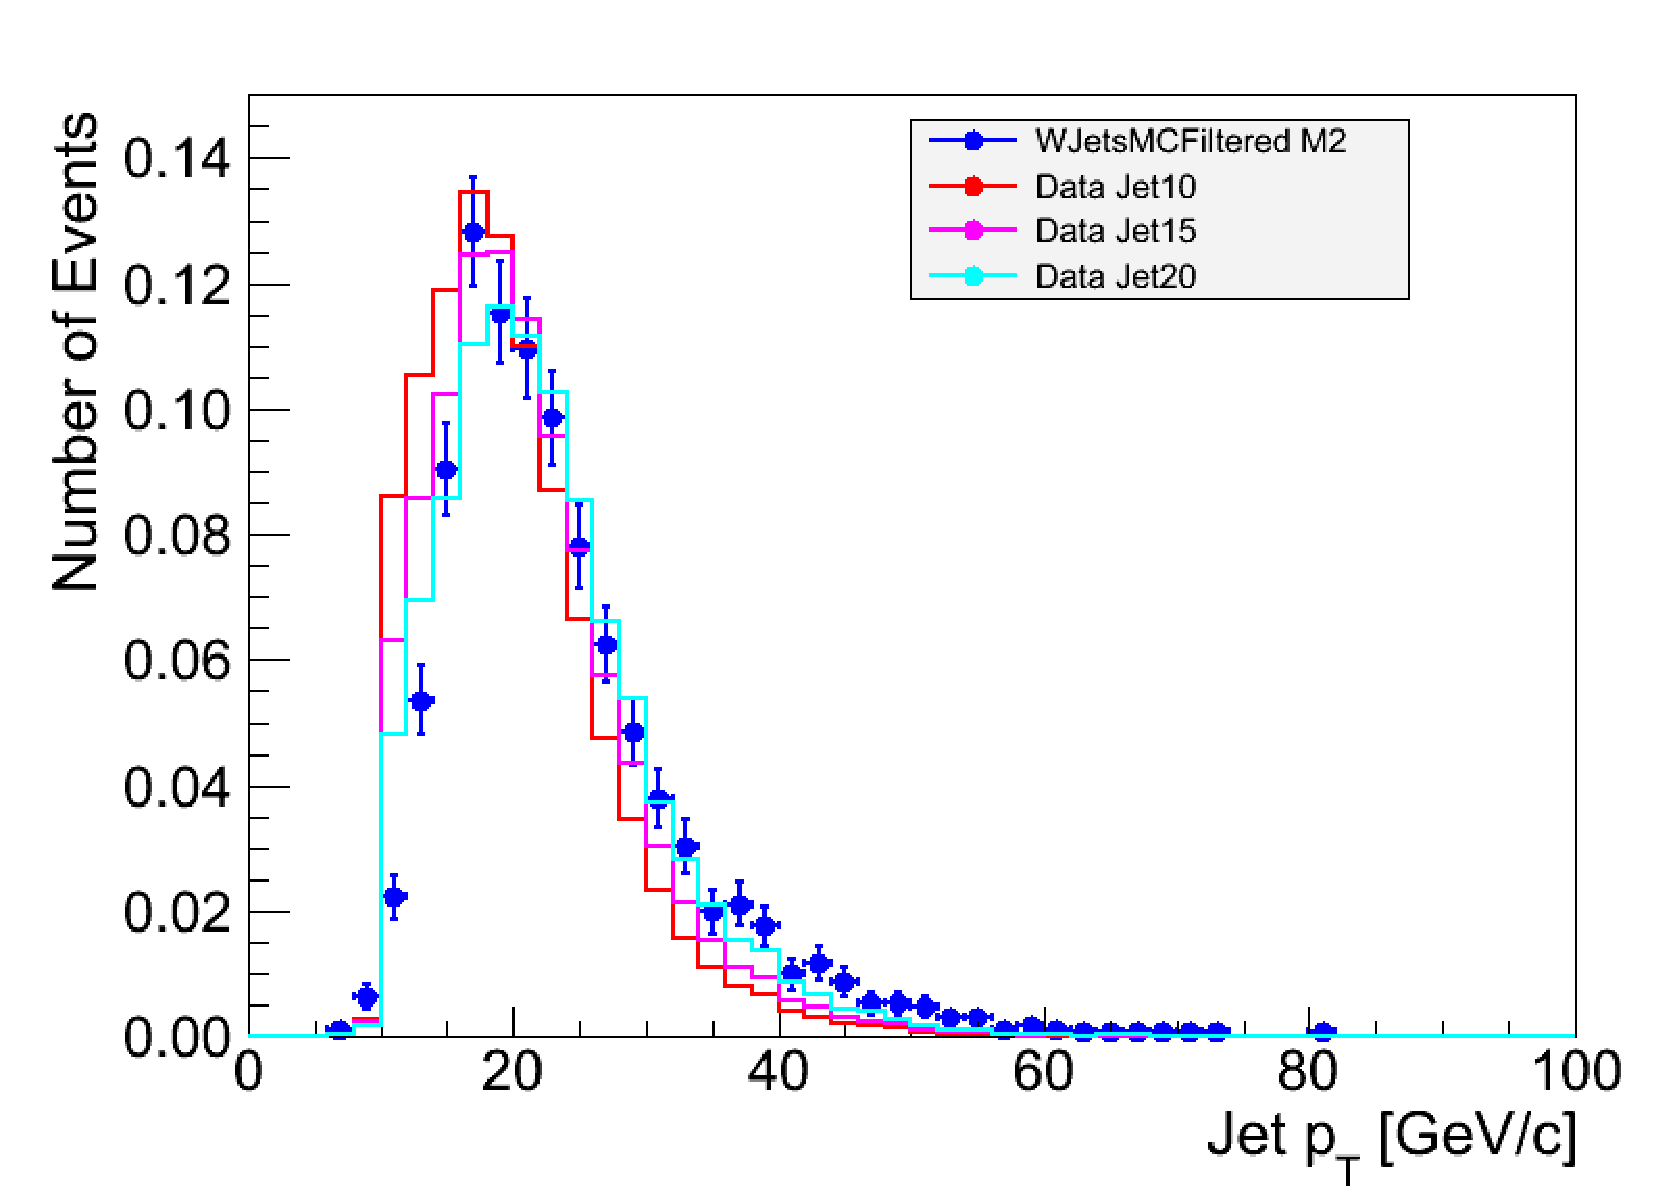
\includegraphics[width=0.45\textwidth]{figures/LeptonJetPt_MuonM2_10To20.pdf}}
\caption{The $p_{T}$ spectrum of the jet that a M2 muon fakeable object lies inside for the 
W+Jet Monte Carlo sample and the data fake rate measurement sample, for a narrower window of thresholds
on the $p_{T}$ of the leading jet in the event.}
\label{fig:mu_M2_fr_jetspectrumNarrowerWindow}
\end{center}
\end{figure}



\begin{table}[!htbp]
\begin{center}
\begin{tabular}{|l|c|c|}
\hline
\multicolumn{3}{|c|}{ M1 Denominator Definition} \\
\hline
                        & \multicolumn{2}{|c|}{ $\%$ Change in Bkg Estimate} \\
\hline
Jet Threshold           & After WW Selection  & After HWW130 Selection \\
\hline
Jet0                    &  $+33\%$     & $+31\%$     \\
Jet5                    &  $+29\%$     & $+28\%$     \\
Jet10                   &  $+20\%$     & $+20\%$     \\
Jet15 (Central Value)   &  $0\%$       & $0\%$       \\
Jet20                   &  $-16\%$     & $-16\%$     \\
Jet25                   &  $-27\%$     & $-33\%$     \\
Jet30                   &  $-41\%$     & $-46\%$     \\
\hline

\hline
\multicolumn{3}{|c|}{ M2 Denominator Definition} \\
\hline
                        & \multicolumn{2}{|c|}{ $\%$ Change in Bkg Estimate} \\
\hline
Jet Threshold           & After WW Selection  & After HWW130 Selection \\
\hline

Jet0                    &  $+19\%$     & $+20\%$     \\
Jet5                    &  $+17\%$     & $+18\%$   \\
Jet10                   &  $+13\%$     & $+14\%$   \\
Jet15 (Central Value)   &  $0\%$       & $0\%$     \\
Jet20                   &  $-8\%$     & $-6\%$     \\
Jet25                   &  $-20\%$     & $-26\%$   \\
Jet30                   &  $-31\%$     & $-40\%$   \\

\hline

\hline
\end{tabular}
\caption{Relative change in the fake muon background estimate using different thresholds on the leading jet to compute the fake rate. }
\label{tab:mu_fr_JetSpectrumSystematics}
\end{center}
\end{table}




 \subsubsection{Sample Extrapolation Systematics and Closure Test}
\label{sec:FakeMuonBkgClosureTest}
 To quantify the systematic uncertainties in extrapolating from the QCD dominated fake rate
calibration sample to the W+Jet dominated application sample, we perform a closure test using 
the Monte Carlo simulation. Fake rates measured from a cross-section weighted combination of 
the QCD Monte Carlo samples, generated with pt-hat $15-30$ GeV and $30-50$ GeV, are applied on
a W+Jet Monte Carlo sample. To measure the fake rate, the selection documented in Section
\ref{sec:MuonFakeRate_CalibrationSampleSelection} is used as in data, with a $p_{T}$ 
threshold of $15$ GeV on the leading jet in the event. These predictions of yields and 
distributions are compared with the yields and distributions obtained from the 
simulation-based result after the WW selection. The sample is normalized to the 
total number of Monte Carlo events in the W+Jet sample, corresponding roughly to $3$ \ifb.
To ensure that we compare only the relevent components of the fake muon background,
we remove any events containing fake electrons. In the subsequent results, 
only the statistical uncertainty from the limited sample size is shown. 
The statistical uncertainty from the limited size of 
the fake rate measurement sample are not propagated. 

Figure \ref{fig:FakeMuonClosureTest_FakeMuPt} shows the comparison of the $p_{T}$
distribution of the fake muon predicted by the fake rate method and the full simulation,
after the dilepton selection and the WW pre-selection. There is remarkably close 
agreement between the prediction using the fake rate method and the simulation
prediction.

\begin{figure}[!htbp]
\begin{center}
\subfigure[After dilepton selection]{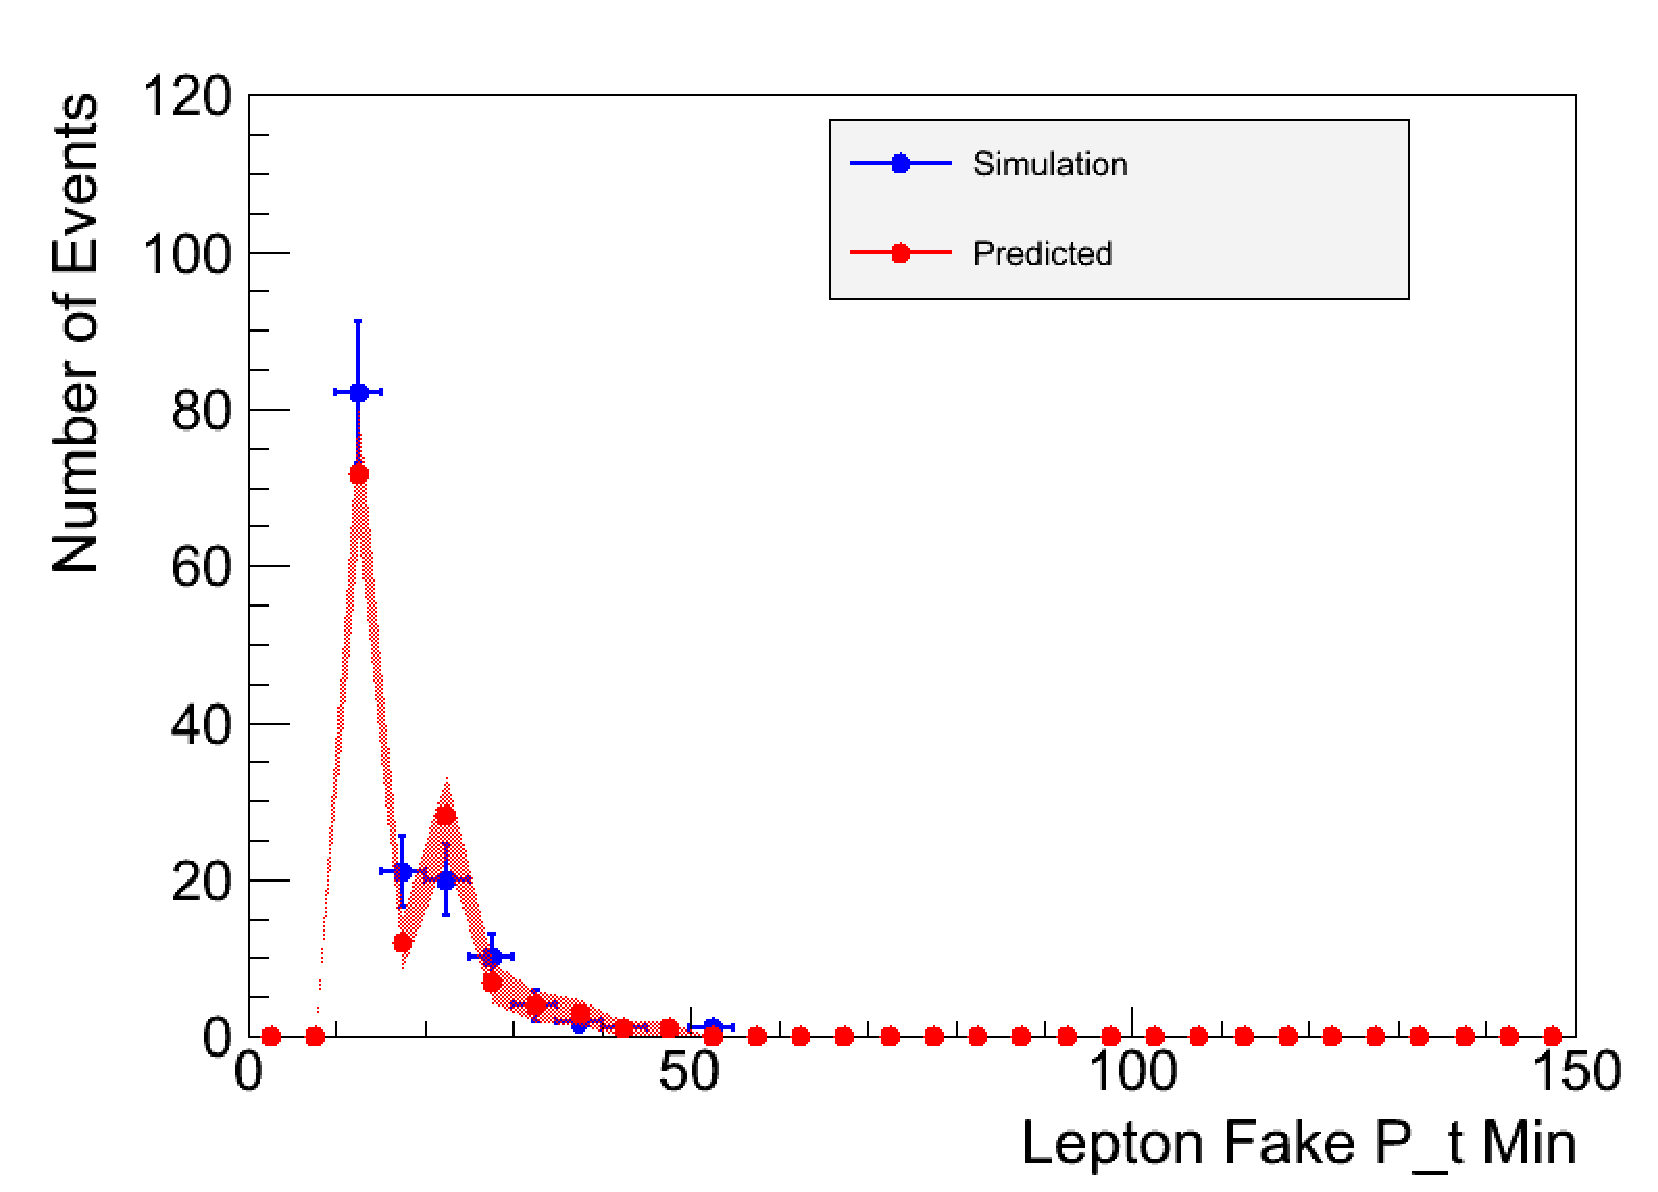
\includegraphics[width=0.45\textwidth]{figures/FakeMuonClosureTest_FakeMuPt_PreSelection.pdf}}
\subfigure[After WW selection]{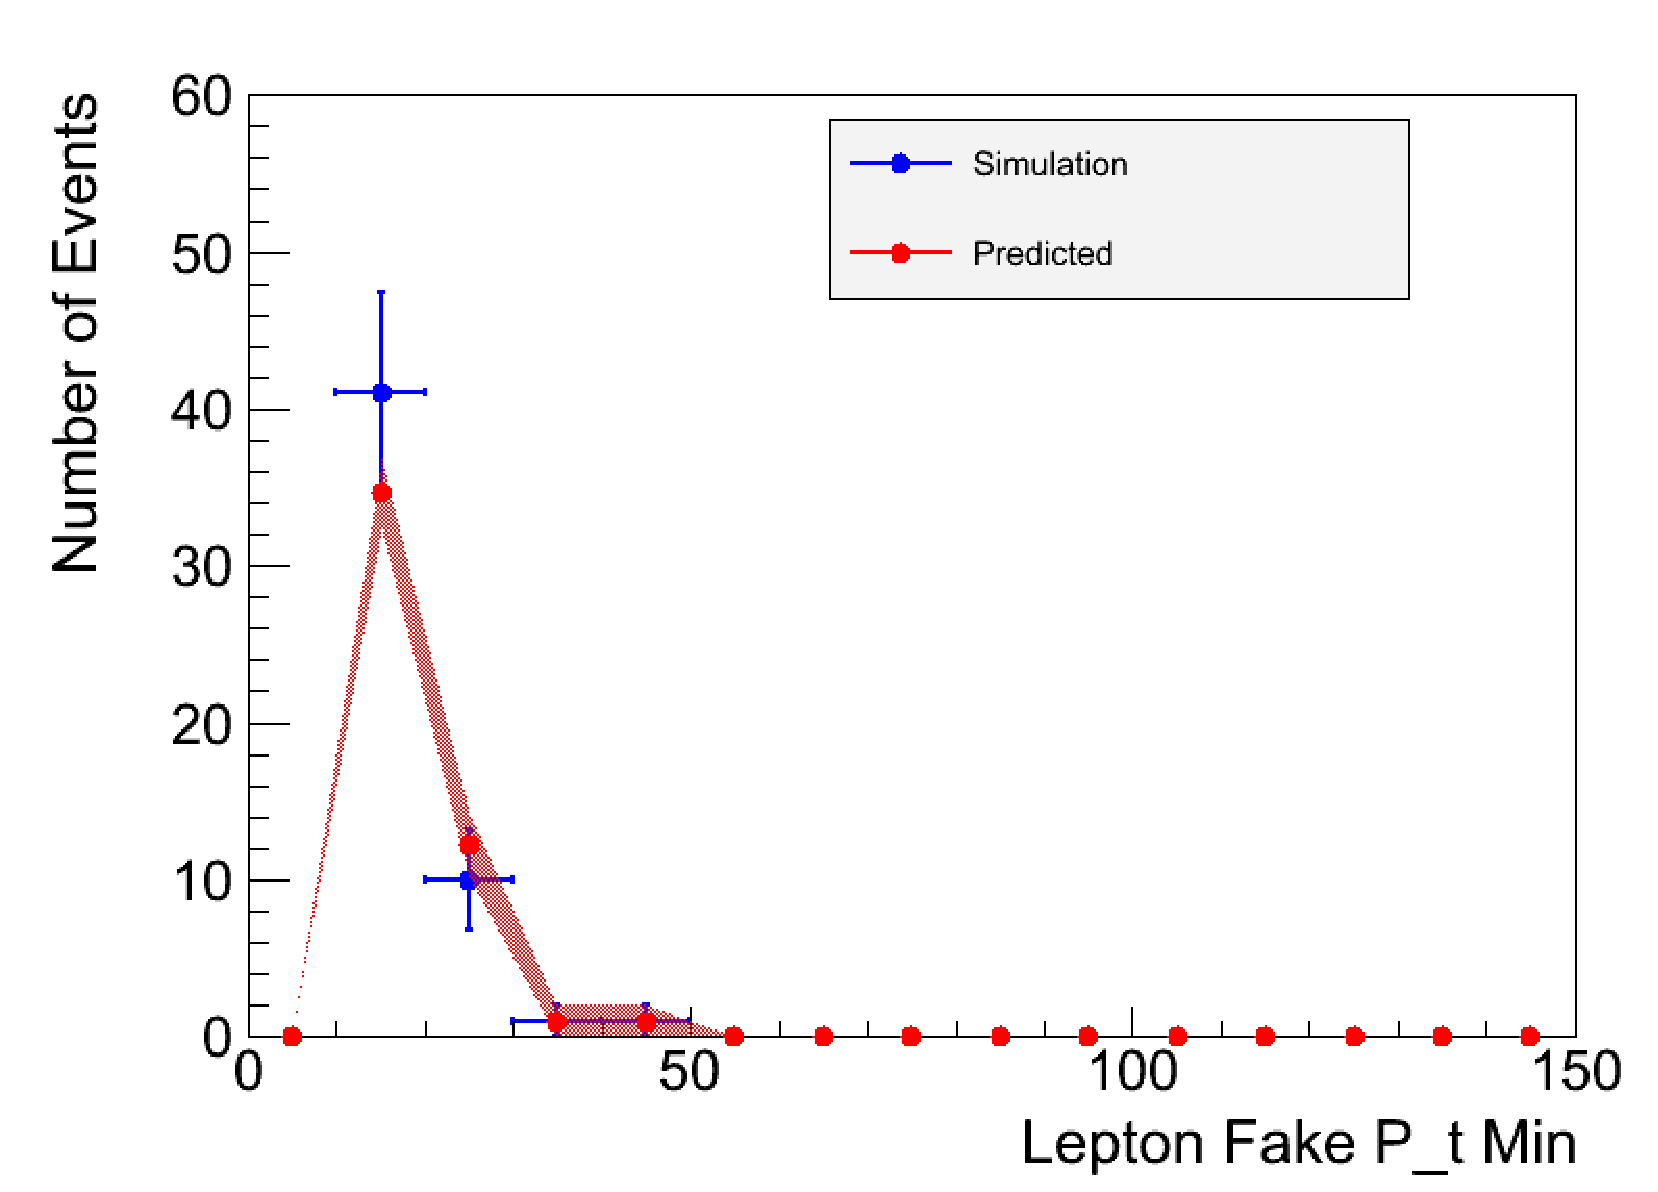
\includegraphics[width=0.45\textwidth]{figures/FakeMuonClosureTest_FakeMuPt.pdf}}
\caption{The $p_{T}$ distribution for the fake muon, after dilepton selection and after
WW selection, is compared between the fake rate method prediction and the simulation prediction. }
\label{fig:FakeMuonClosureTest_FakeMuPt}
\end{center}
\end{figure}

Table \ref{tab:FakeMuonClosureTest_Yields} summarizes the comparison between the
predicted yields and the yields from the Monte Carlo simulation, at various stages
of the Higgs selection. At all stages of the selection, the relative difference
between the predicted yield and the simulated yield is less than $20\%$.

\begin{table}[!htbp]
\begin{center}
\begin{tabular}{|l|c|c|c|}
\hline
\multicolumn{4}{|c|}{After dilepton selection} \\
\hline
Final State     & Predicted Yield   & Simulation Yield & Fractional Difference\\
\hline
$\mu\mu$        &  $96 \pm 5$      & $102 \pm 10$     & $-6\%$\\
e $\mu$         &  $76 \pm 4$      & $71 \pm 8$       & $+7\%$\\
total           &  $172 \pm 7$     & $173 \pm 13$     & $-1\%$\\
\hline
\multicolumn{4}{|c|}{After dilepton selection and $\met > 20$ GeV, $M_{\mathrm{ll}} > 12$ GeV cuts} \\
\hline
Final State     & Predicted Yield   & Simulation Yield & Fractional Difference\\
\hline
$\mu\mu$        &  $71 \pm 4$      & $85 \pm 9$     & $-16\%$\\
e $\mu$         &  $59 \pm 4$      & $60 \pm 7$     & $-2\%$\\
total           &  $130 \pm 6$     & $145 \pm 12$   & $-10\%$\\
\hline
\multicolumn{4}{|c|}{After WW selection} \\
\hline
Final State     & Predicted Yield   & Simulation Yield & Fractional Difference\\
\hline
$\mu\mu$        &  $16.5 \pm 1.9$  & $20 \pm 4.5$   & $-18\%$  \\
e $\mu$         &  $33.8 \pm 2.8$  & $35 \pm 5.9$   & $-3\%$  \\
total           &  $50.3 \pm 3.4$  & $55 \pm 7.4$   & $-9\%$  \\
\hline
\multicolumn{4}{|c|}{After HWW 130 selection} \\
\hline
Final State     & Predicted Yield   & Simulation Yield & Fractional Difference\\
\hline
$\mu\mu$        &  $3.6 \pm 0.8$   & $3 \pm 1.7$     & $+20\%$\\
e $\mu$         &  $4.1 \pm 0.8$   & $5 \pm 2.2$     & $-18\%$\\
total           &  $7.7 \pm 1.1$   & $8 \pm 2.8$     & $-4\%$\\
\hline
\end{tabular}
\caption{Comparison of fake muon background yields at various stages of the 
analysis selection between the fake rate method prediction and the simulation
prediction. }
\label{tab:FakeMuonClosureTest_Yields}
\end{center}
\end{table}

Figure \ref{fig:FakeMuonClosureTest_LeptonPt} shows the comparison of the $p_{T}$
of the leading and trailing leptons after the WW selection between the prediction
from the fake rate method and from the simulation. Analogous comparisons for 
the missing transverse energy, the $\Delta\phi$ between the two leptons, 
the dilepton mass, and the transverse mass of the Higgs are shown in 
Figures \ref{fig:FakeMuonClosureTest_MetAndDeltaPhi} and 
\ref{fig:FakeMuonClosureTest_MetAndDeltaPhi}. We do not observe any statistically 
significant systematic differences in the shapes of any of these distributions. Finally, 
Figure \ref{fig:FakeMuonClosureTest_CutFlow} shows the comparison of the 
cut flow for the $ee$ and $e\mu$ final states between
the prediction from the fake rate method and the simulation. Again, no major 
discrepancies beyond the $20\%$ level are observed. 


\begin{figure}[!htbp]
\begin{center}
\subfigure[Leading lepton $p_{T}$]{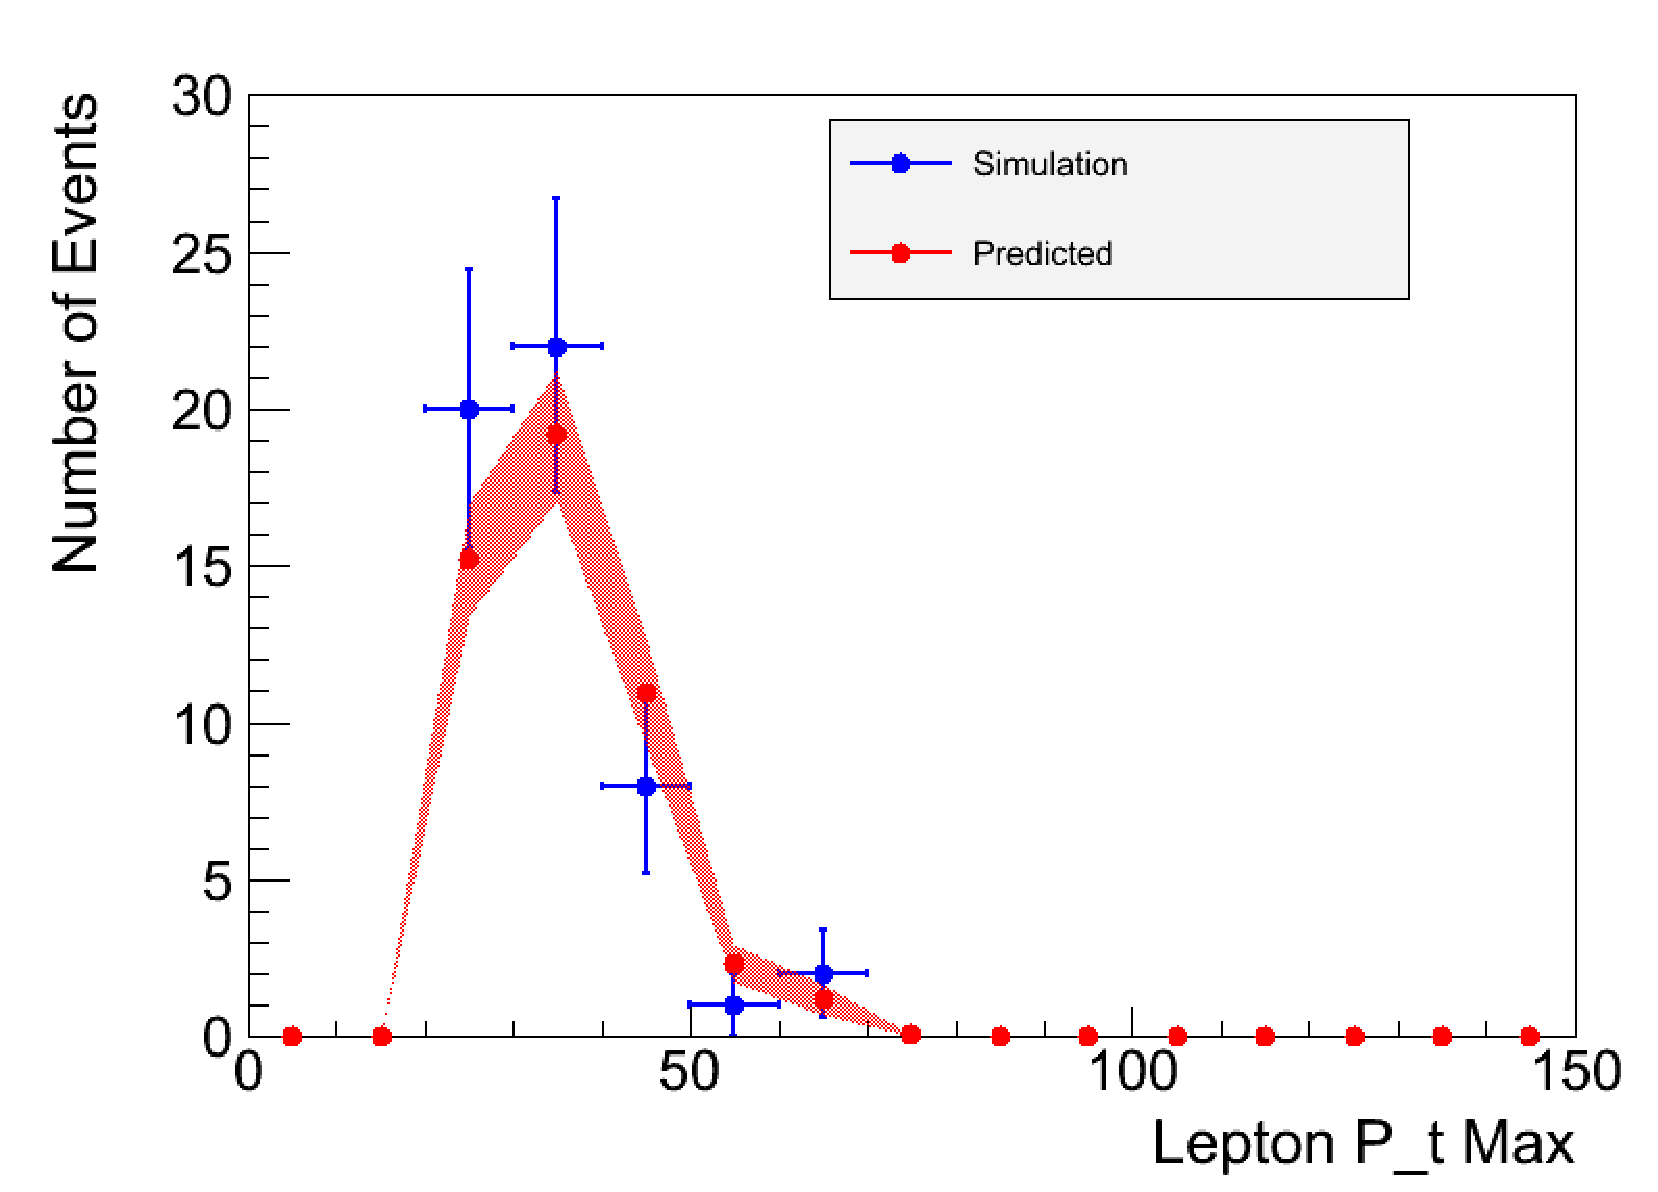
\includegraphics[width=0.45\textwidth]{figures/FakeMuonClosureTest_PtMax.pdf}}
\subfigure[Trailing lepton $p_{T}$]{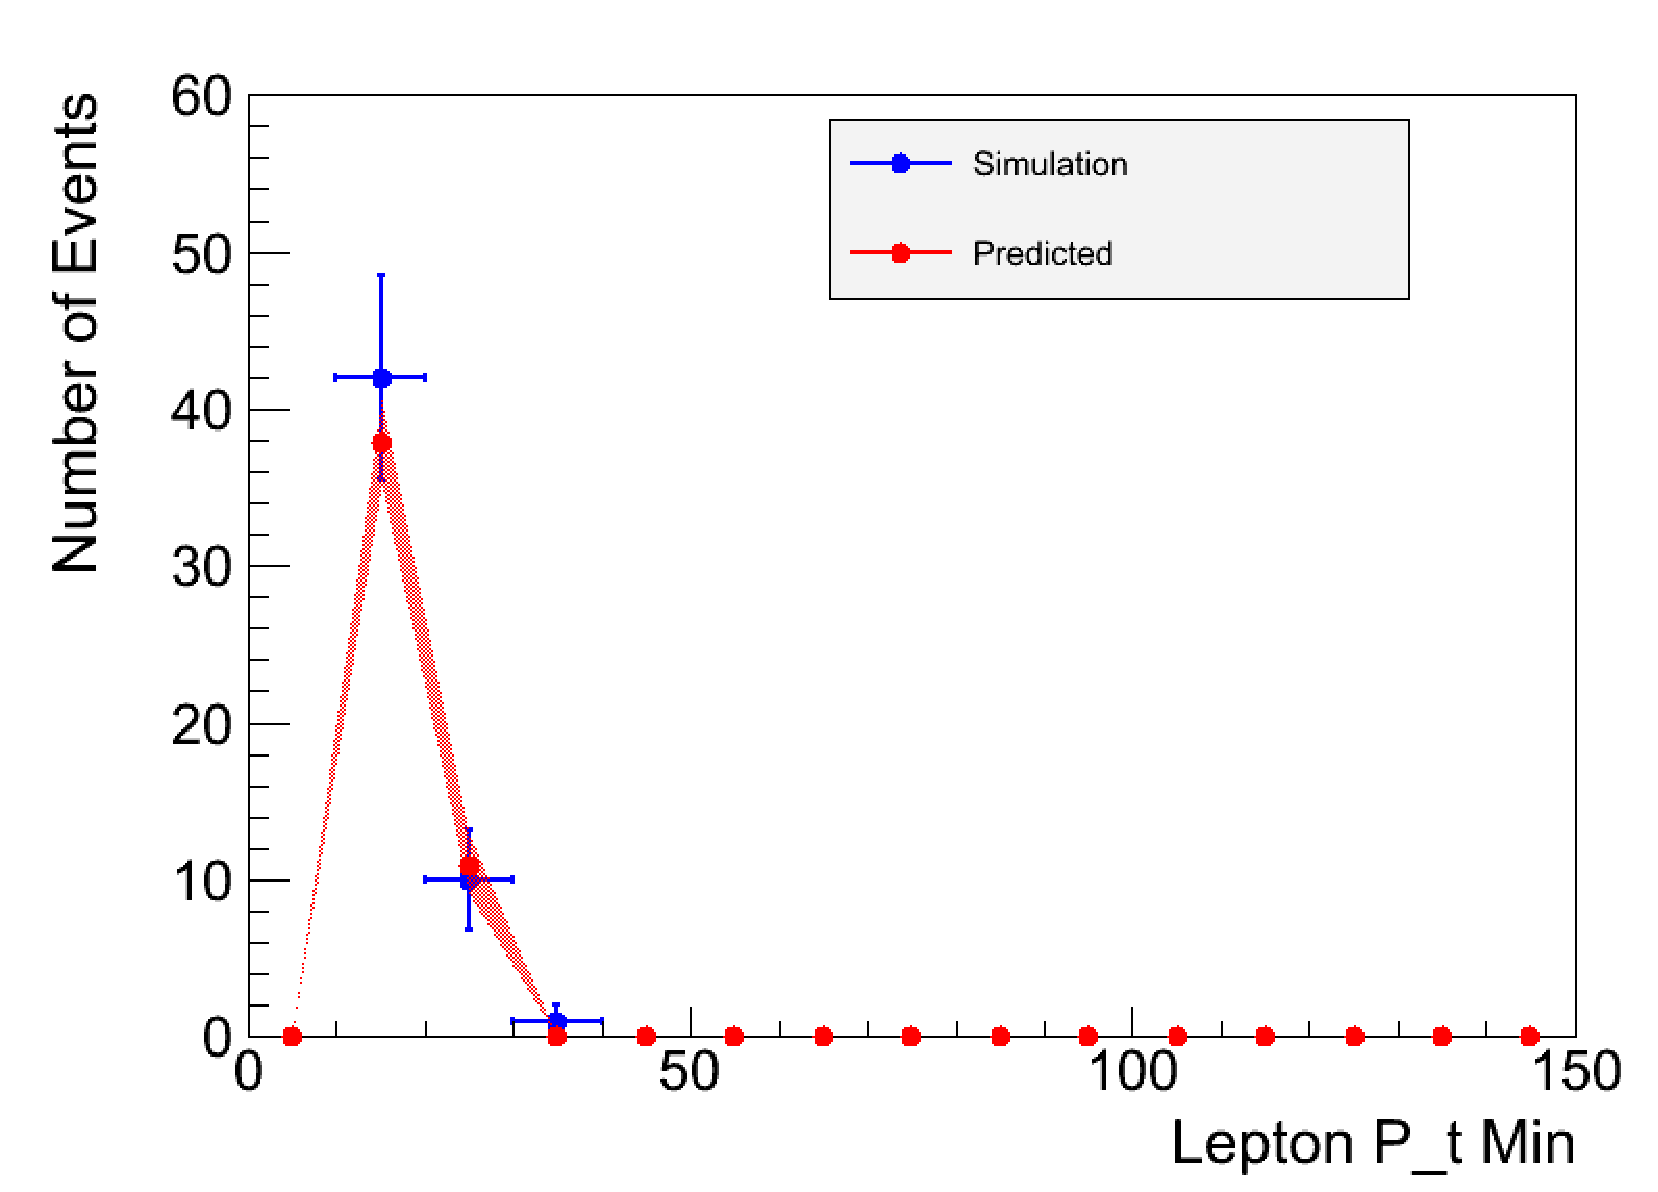
\includegraphics[width=0.45\textwidth]{figures/FakeMuonClosureTest_PtMin.pdf}}
\caption{A comparison of the $p_{T}$ distribution of the leading and trailing lepton
between the fake rate method prediction and the simulation prediction. }
\label{fig:FakeMuonClosureTest_LeptonPt}
\end{center}
\end{figure}

\begin{figure}[!htbp]
\begin{center}
\subfigure[$\met$]{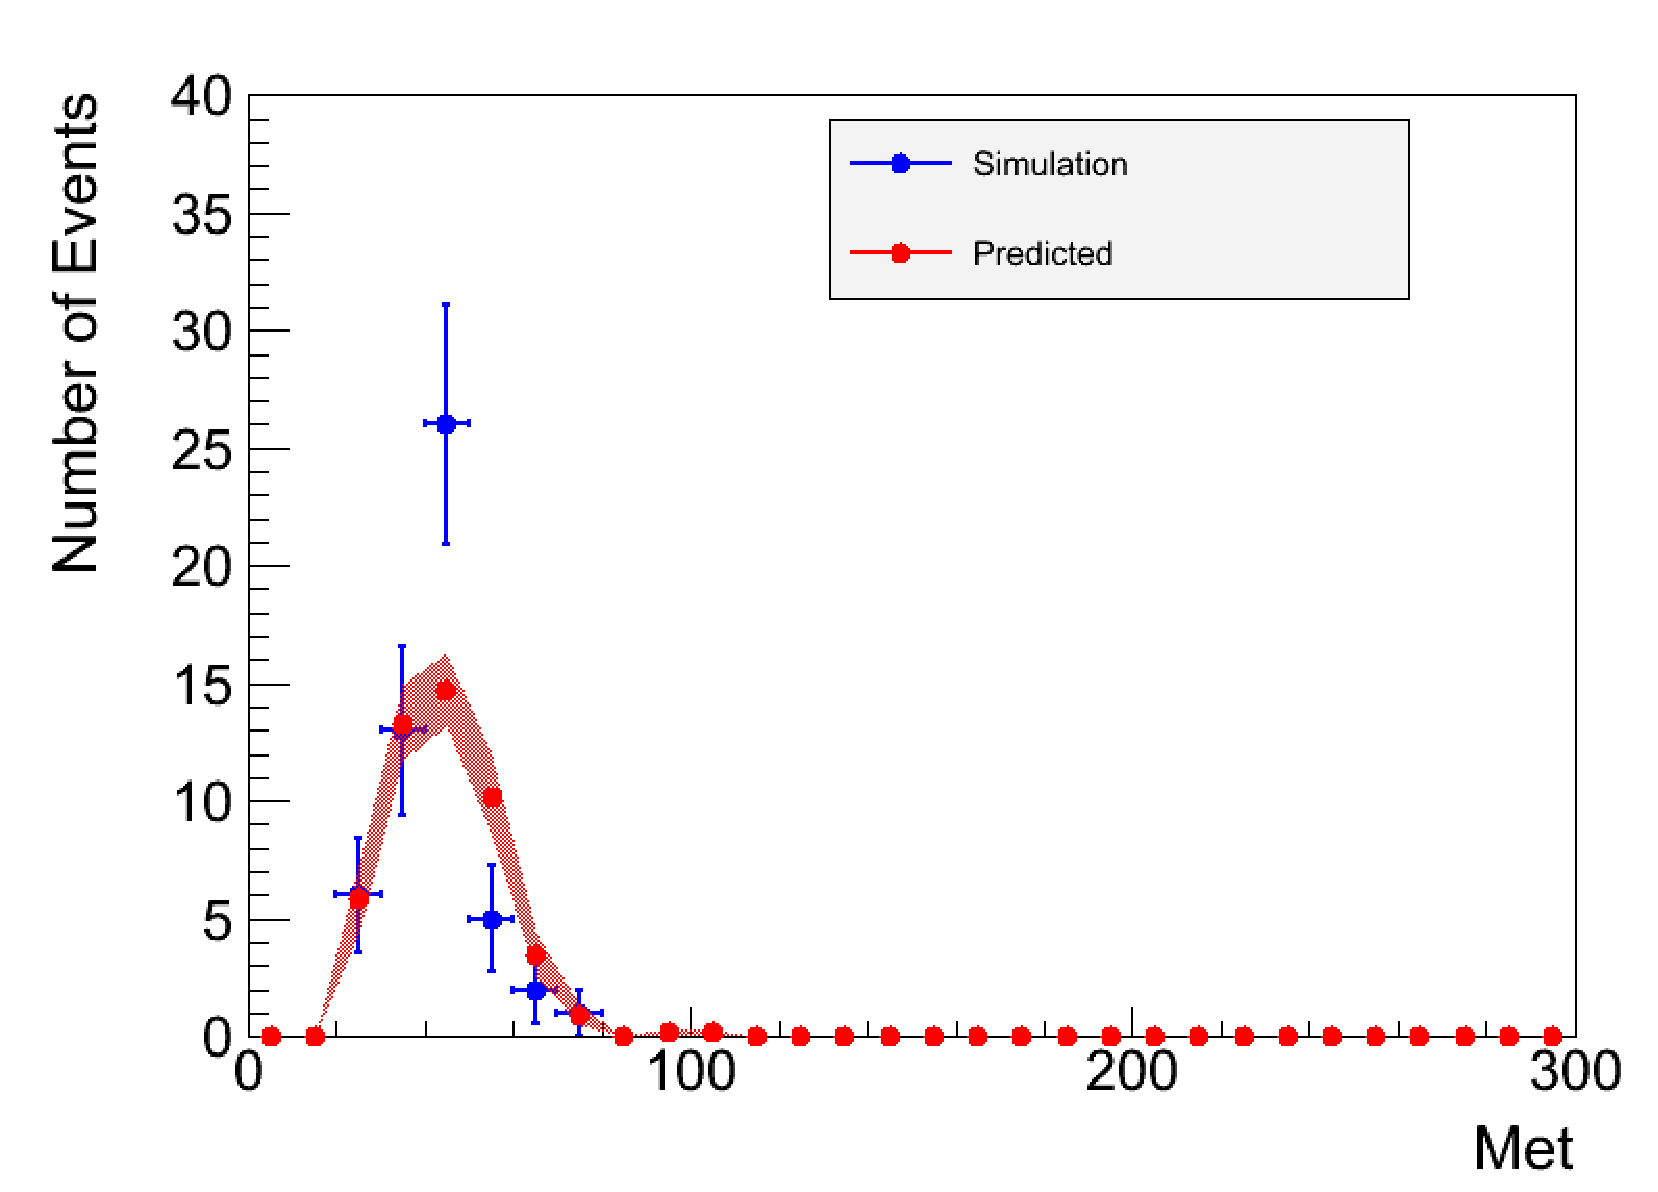
\includegraphics[width=0.45\textwidth]{figures/FakeMuonClosureTest_Met.pdf}}
\subfigure[$\Delta\phi$]{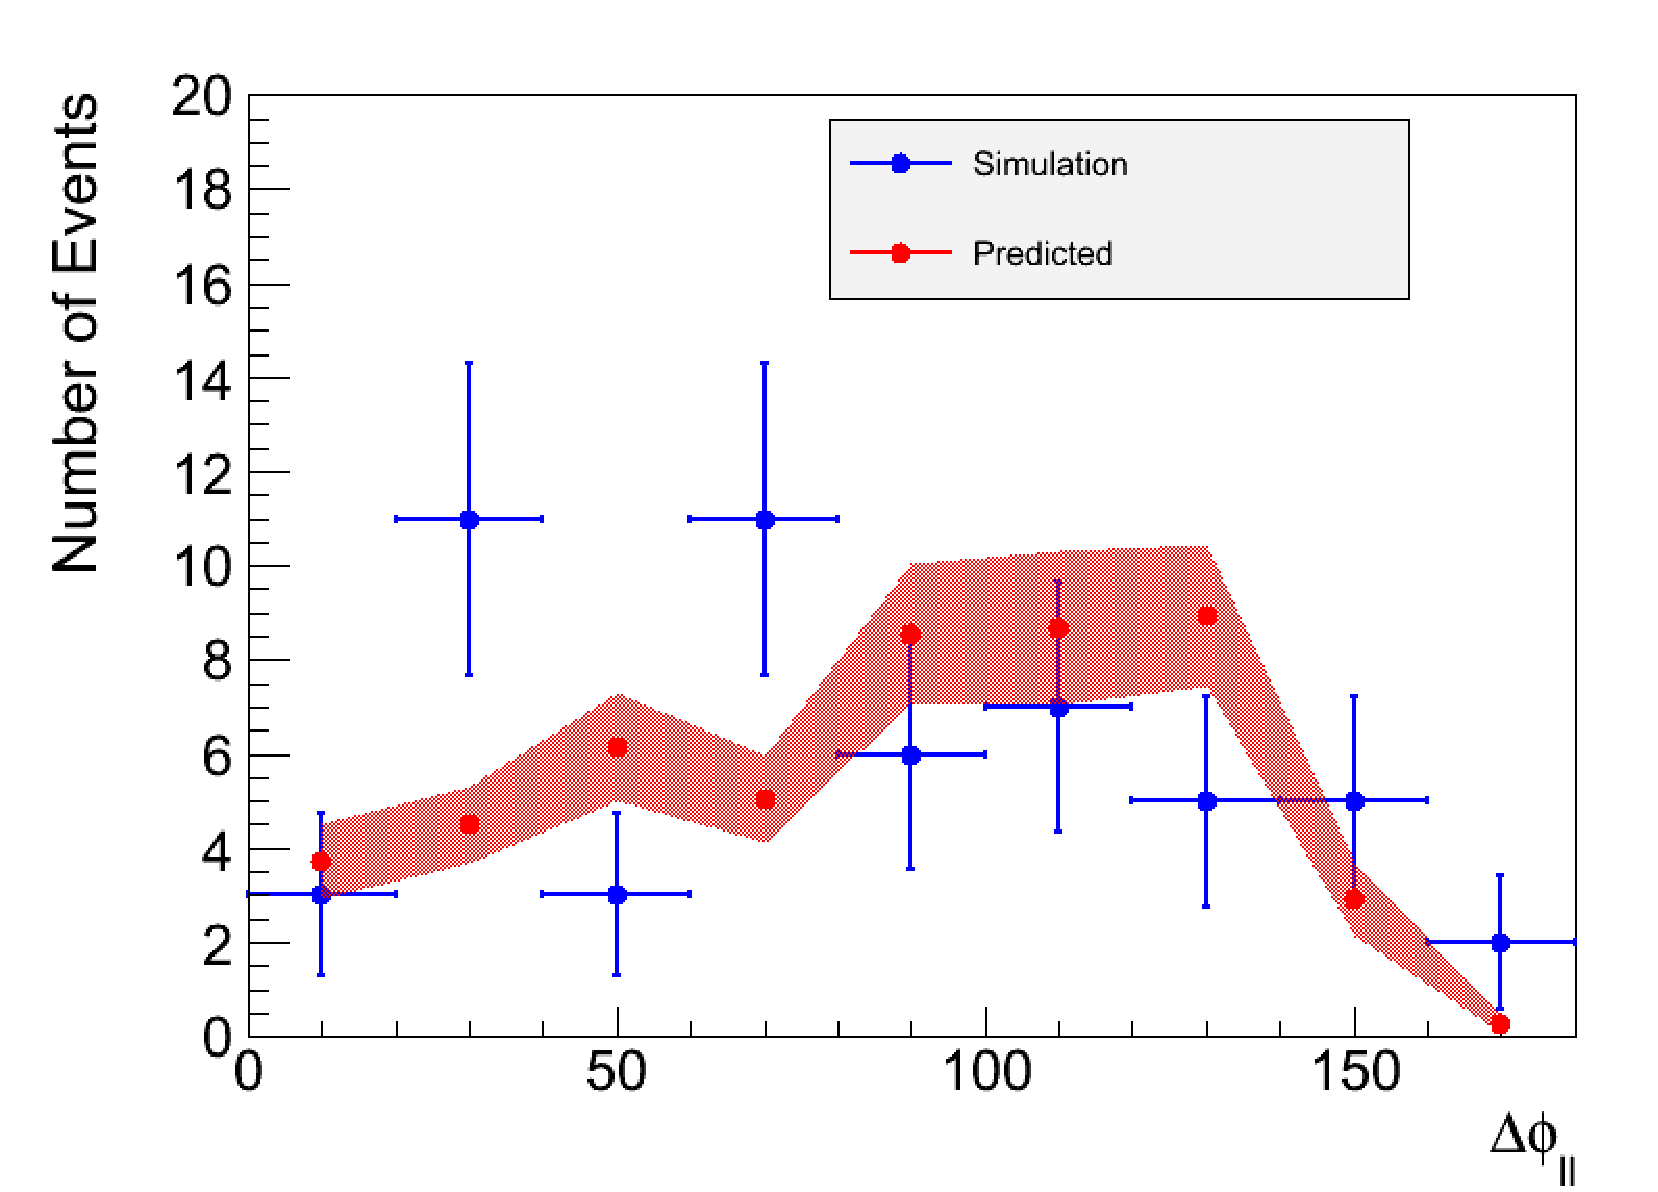
\includegraphics[width=0.45\textwidth]{figures/FakeMuonClosureTest_DeltaPhi.pdf}}
\caption{A comparison of the distribution of the missing transverse energy, 
and the $\Delta\phi$ between the two leptons predicted using the fake rate method and the
full simulation.}
\label{fig:FakeMuonClosureTest_MetAndDeltaPhi}
\end{center}
\end{figure}

\begin{figure}[!htbp]
\begin{center}
\subfigure[Dilepton Mass]{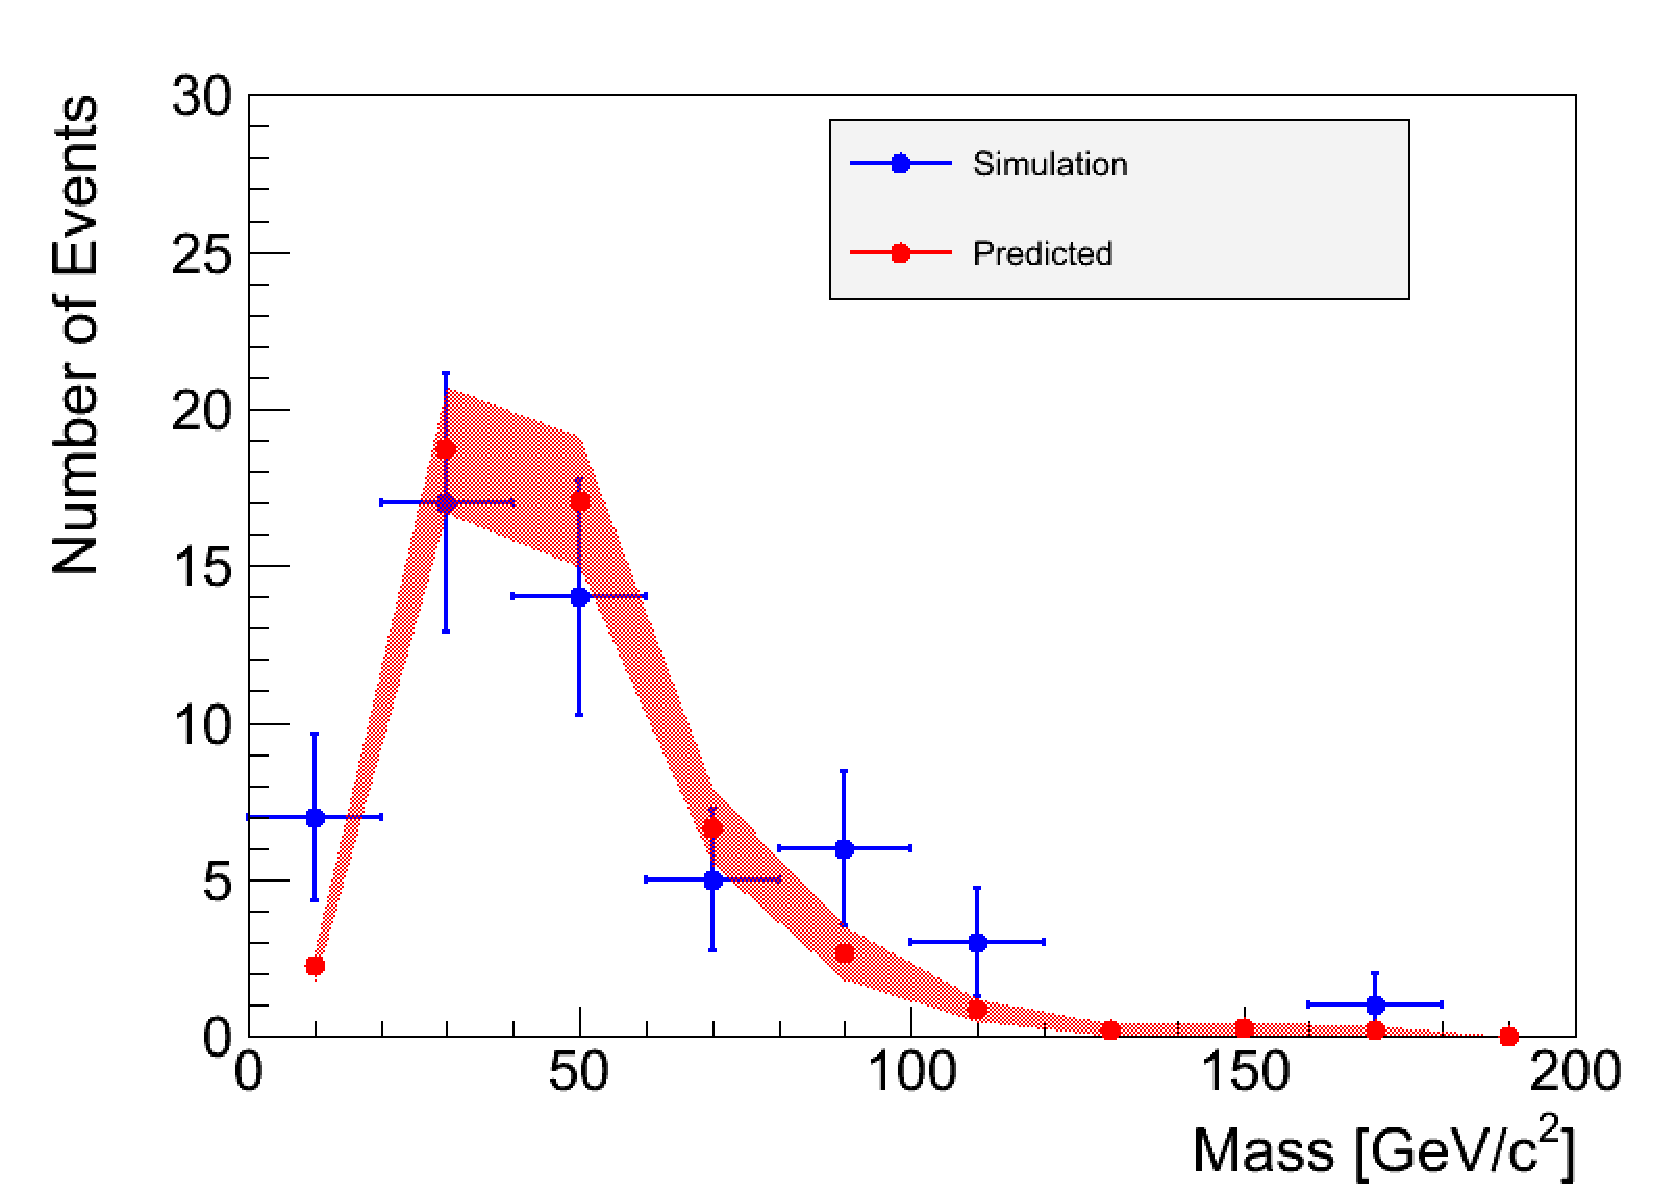
\includegraphics[width=0.45\textwidth]{figures/FakeMuonClosureTest_DileptonMass.pdf}}
\subfigure[Higgs $M_{T}$]{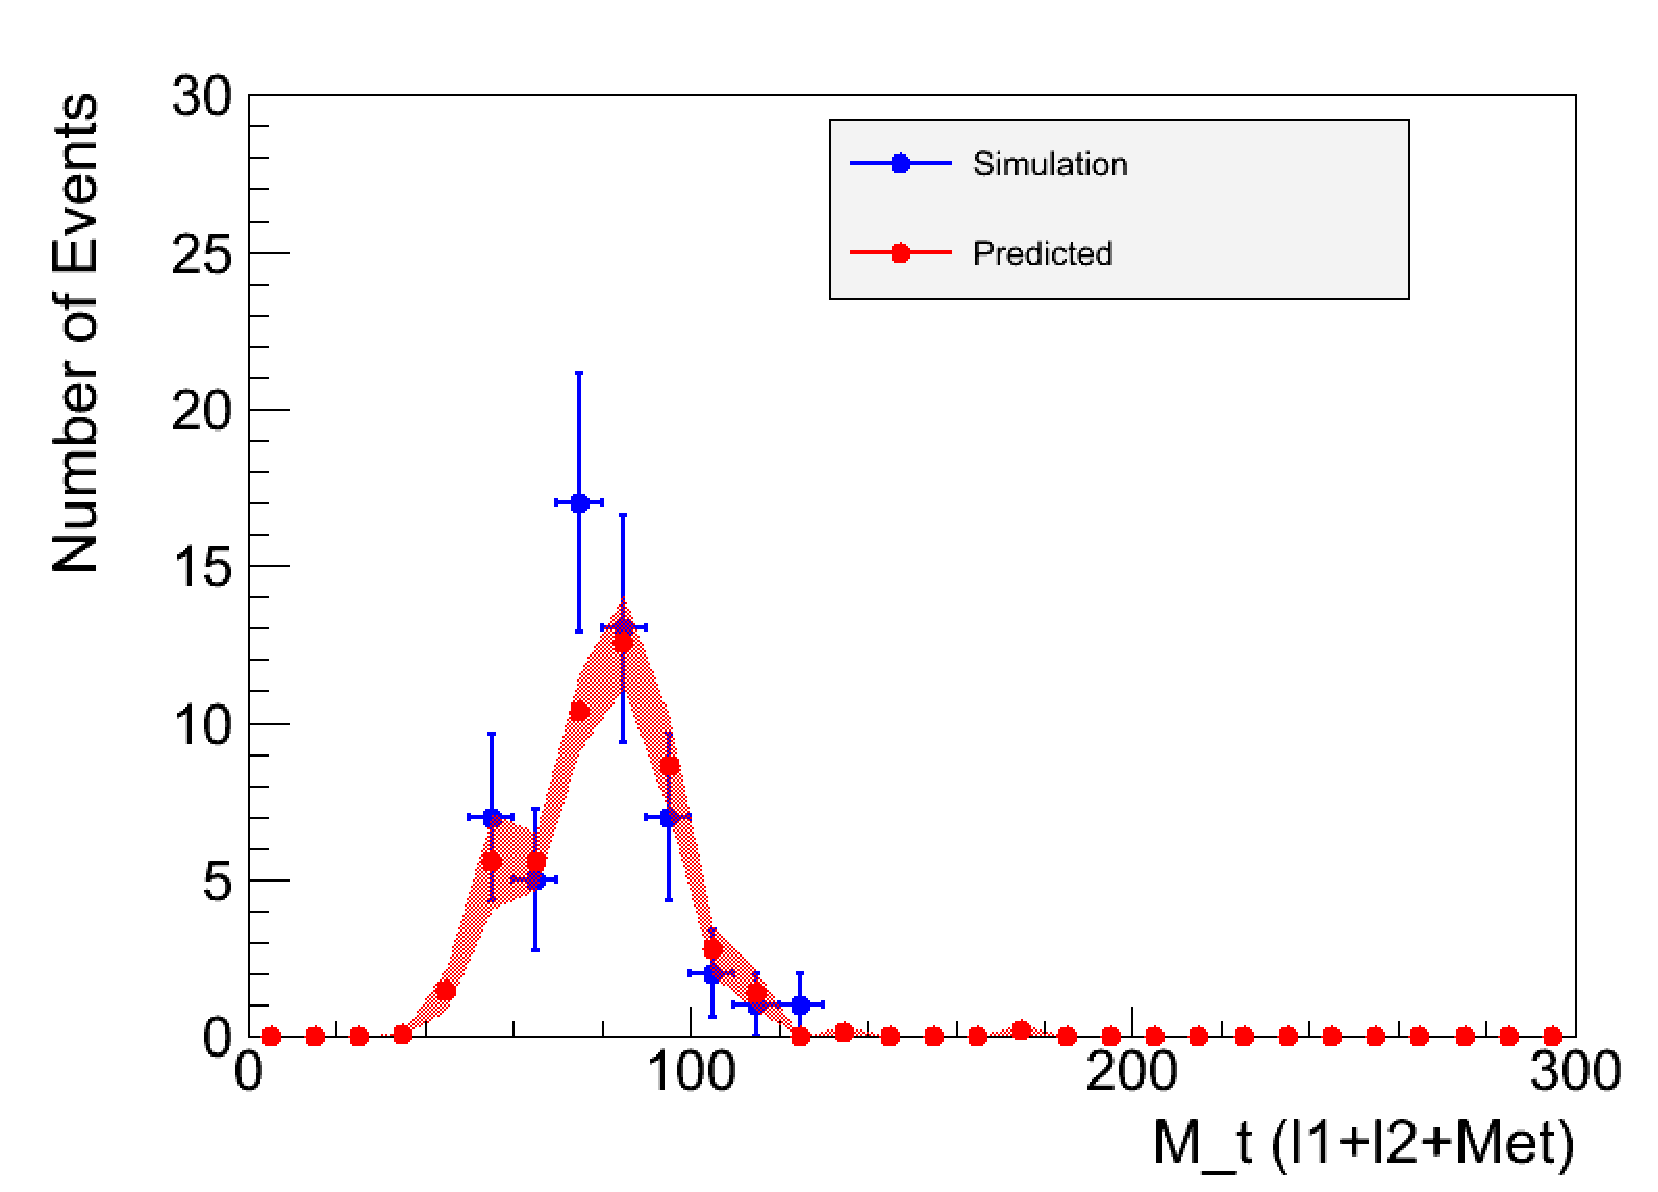
\includegraphics[width=0.45\textwidth]{figures/FakeMuonClosureTest_MtHiggs.pdf}}
\caption{A comparison of the distribution of the dilepton mass and Higgs transverse mass 
predicted using the fake rate method and the full simulation.}
\label{fig:FakeMuonClosureTest_DileptonMassAndMtHiggs}
\end{center}
\end{figure}


\begin{figure}[!htbp]
\begin{center}
\subfigure[ee]{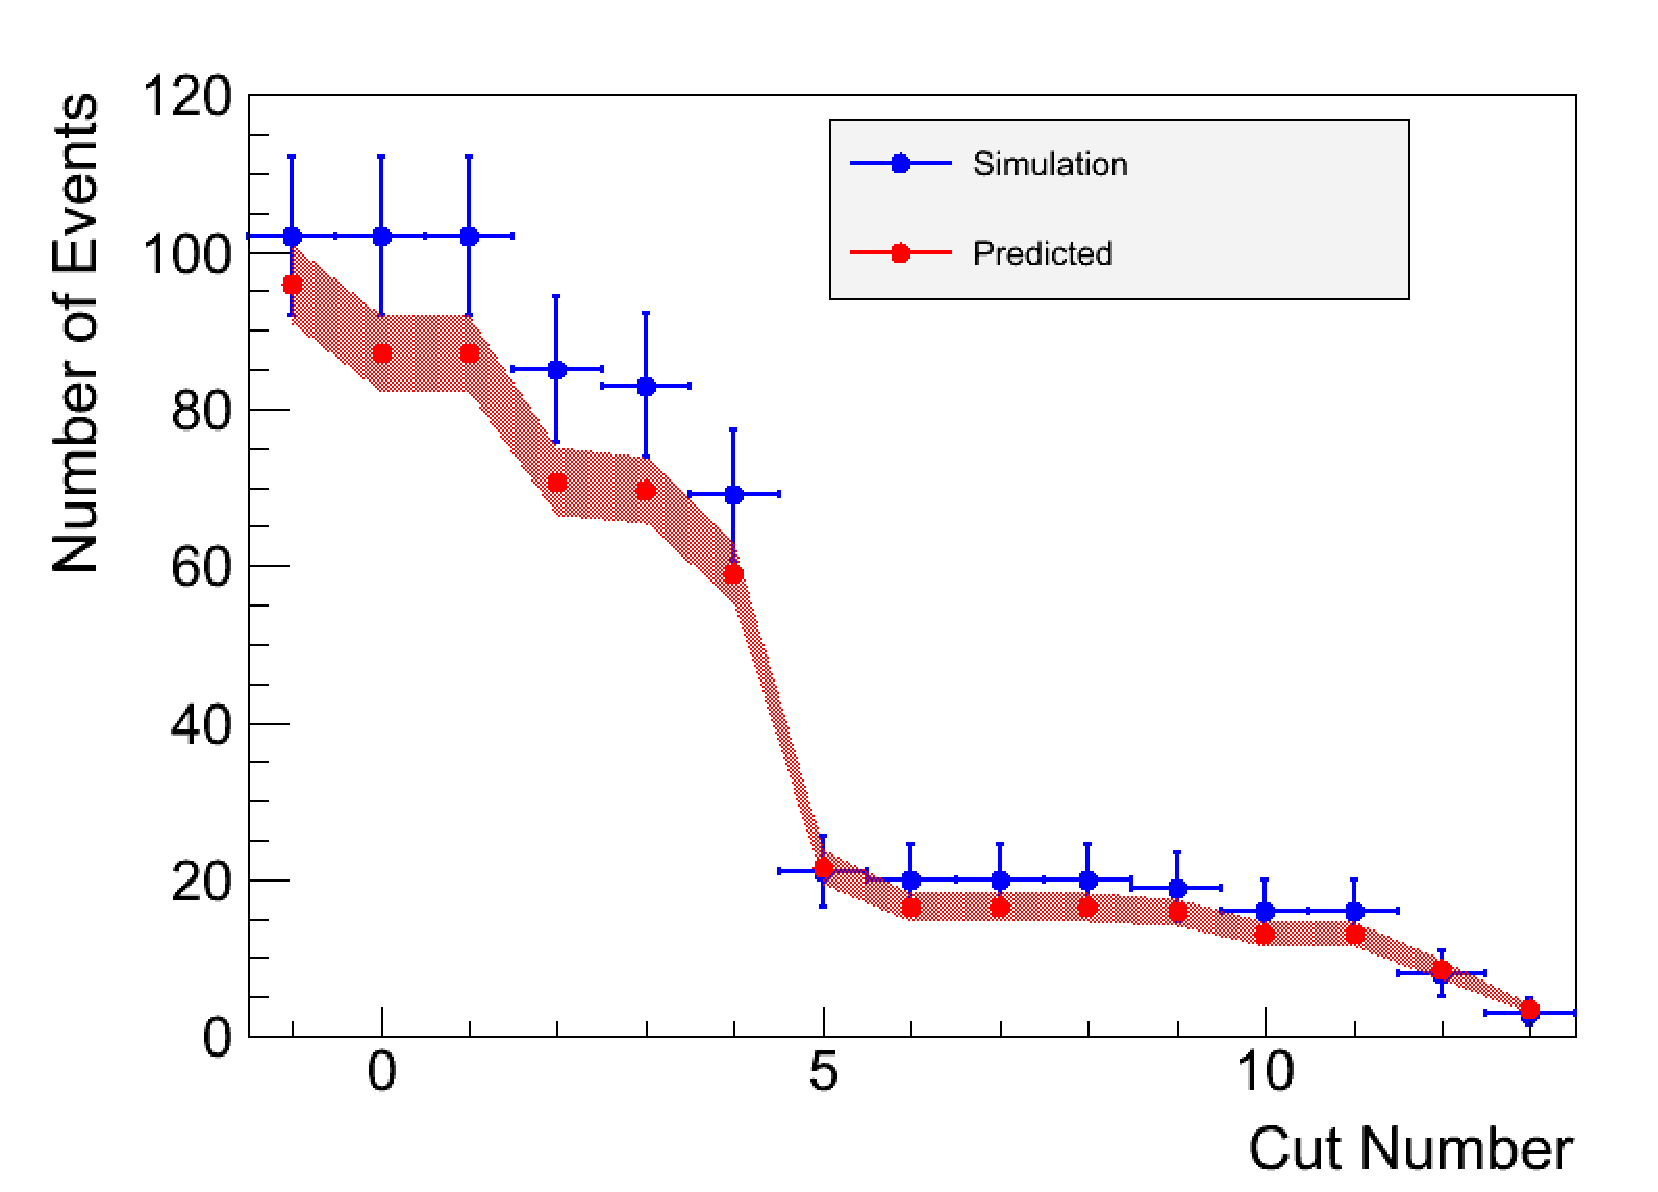
\includegraphics[width=0.45\textwidth]{figures/FakeMuonClosureTest_CutFlowMuMu.pdf}}
\subfigure[e$\mu$]{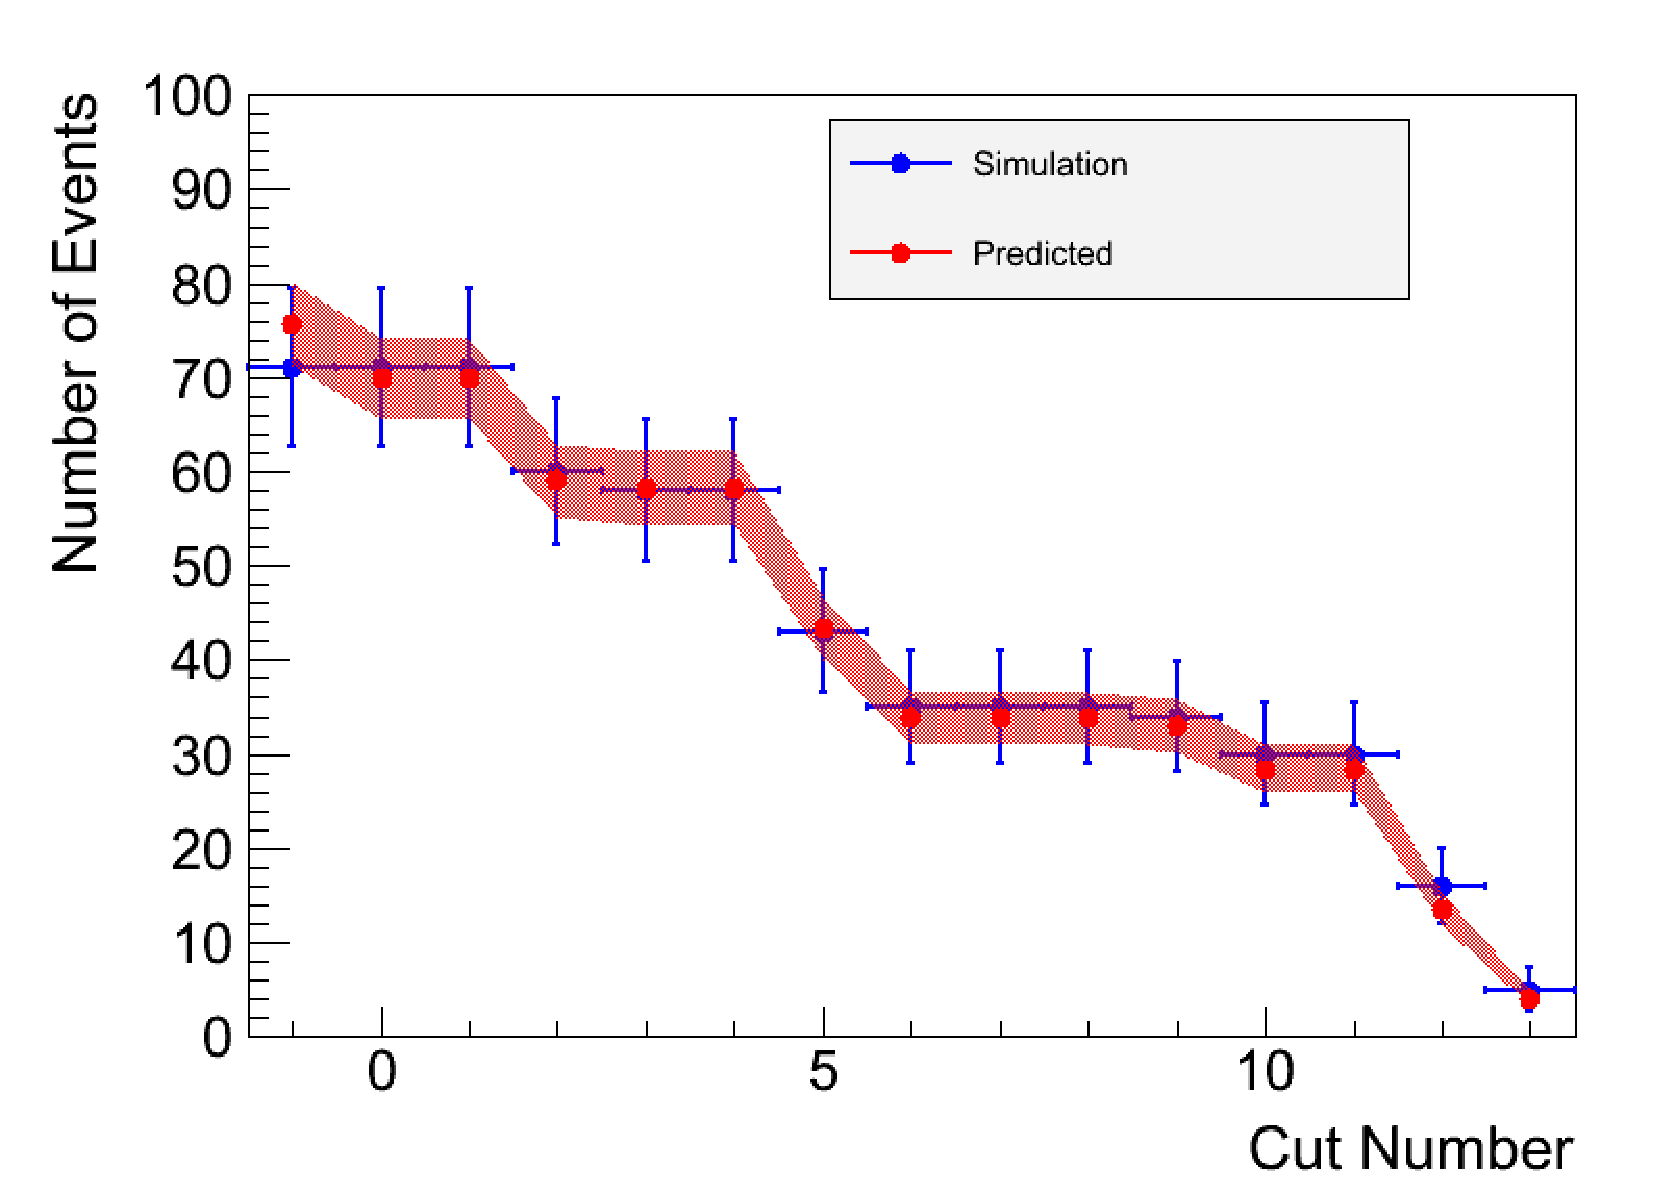
\includegraphics[width=0.45\textwidth]{figures/FakeMuonClosureTest_CutFlowEMu.pdf}}
\caption{A comparison of the cut flow of the W+Jet background for the ee and e$\mu$ final states
between the fake rate method prediction and the full simulation prediction. }
\label{fig:FakeMuonClosureTest_CutFlow}
\end{center}
\end{figure}

To summarize, ignoring the yield comparison after the final Higgs selection cuts which 
suffer from large statistical uncertainties, we estimate a systematic uncertainty of 
$18\%$ for the fake muon background prediction due to the sample extrapolation 
coming from the largest differences observed in the yields of the closure test from 
Table \ref{tab:FakeMuonClosureTest_Yields}. 

